\documentclass[12pt, a4paper]{report}

% ── Packages ──────────────────────────────────────────────────
\usepackage[utf8]{inputenc}
\usepackage[T1]{fontenc}
\usepackage[english]{babel}
\usepackage{times}                      % Times New Roman
\usepackage[
  top=3cm, bottom=3cm,
  left=3.5cm, right=2.5cm            % NEU standard margins
]{geometry}
\usepackage{setspace}
\onehalfspacing                         % 1.5 line spacing

\usepackage{graphicx}
\usepackage{float}
\usepackage{booktabs}
\usepackage{longtable}
\usepackage{caption}
\usepackage{subcaption}
\usepackage{amsmath, amssymb}
\usepackage{listings}                   % code blocks
\usepackage{xcolor}
\usepackage{hyperref}
\usepackage[round, authoryear]{natbib}  % APA author-year (Smith, 2020)
\usepackage{fancyhdr}
\usepackage{titlesec}
\usepackage{tocloft}
\usepackage{acronym}
\usepackage{multirow}
\usepackage{array}
\usepackage{tikz}                       % for title-page border
\usepackage{seqsplit}                   % break overlong \texttt strings
\usepackage{microtype}                  % Globally fixes overfull hboxes
\tolerance=1000
\emergencystretch=1.5em                 % Allows slight word spacing stretching

% ── Hyperref setup ────────────────────────────────────────────
\hypersetup{
  colorlinks=true,
  linkcolor=black,
  citecolor=black,
  urlcolor=blue,
  pdftitle={Amazon Marketplace Intelligence: A Data-Driven Framework for Competitive Monitoring of Consumer Electronics},
  pdfauthor={Nguyen Thi Mai Linh},
}

% ── Chapter title style ───────────────────────────────────────
% NEU DSEB convention: "CHAPTER N: TITLE" on a single line, centered, bold.
\titleformat{\chapter}[hang]
  {\normalfont\Large\bfseries\centering}
  {CHAPTER \thechapter:}{0.5em}{}
\titlespacing*{\chapter}{0pt}{-20pt}{24pt}

% Section numbering with trailing period: 1.1. , 1.1.1. , 1.1.1.1.
\titleformat{\section}
  {\normalfont\large\bfseries}
  {\thesection.}{0.5em}{}
\titleformat{\subsection}
  {\normalfont\normalsize\bfseries}
  {\thesubsection.}{0.5em}{}
\titleformat{\subsubsection}
  {\normalfont\normalsize\bfseries\itshape}
  {\thesubsubsection.}{0.5em}{}

% ── Table of Contents style (NEU DSEB convention) ─────────────
\renewcommand{\contentsname}{TABLE OF CONTENTS}
\addto\captionsenglish{\renewcommand{\contentsname}{TABLE OF CONTENTS}}

% Chapter line: "CHAPTER N: TITLE" in bold caps with dotted leader
\renewcommand{\cftchapfont}{\normalfont\bfseries\MakeUppercase}
\renewcommand{\cftchappagefont}{\normalfont\bfseries}
\renewcommand{\cftchappresnum}{CHAPTER\ }
\renewcommand{\cftchapaftersnum}{:}
\setlength{\cftchapnumwidth}{6.5em}

% Section: "1.1. Title" bold
\renewcommand{\cftsecfont}{\normalfont\bfseries}
\renewcommand{\cftsecpagefont}{\normalfont}
\renewcommand{\cftsecaftersnum}{.}
\setlength{\cftsecindent}{1.5em}
\setlength{\cftsecnumwidth}{2.8em}

% Subsection: "1.1.1. Title" italic
\renewcommand{\cftsubsecfont}{\normalfont\itshape}
\renewcommand{\cftsubsecpagefont}{\normalfont}
\renewcommand{\cftsubsecaftersnum}{.}
\setlength{\cftsubsecindent}{3.5em}
\setlength{\cftsubsecnumwidth}{3.4em}

% Dotted leaders for all levels
\renewcommand{\cftdotsep}{1.5}
\renewcommand{\cftchapleader}{\cftdotfill{\cftdotsep}}
\renewcommand{\cftsecleader}{\cftdotfill{\cftdotsep}}
\renewcommand{\cftsubsecleader}{\cftdotfill{\cftdotsep}}
\setlength{\cftbeforechapskip}{4pt}
\setlength{\cftbeforesecskip}{2pt}
\setlength{\cftbeforesubsecskip}{2pt}

% Center the TOC heading
\renewcommand{\cfttoctitlefont}{\normalfont\Large\bfseries\centering}
\renewcommand{\cftaftertoctitle}{}

% ── Header/Footer ─────────────────────────────────────────────
\pagestyle{fancy}
\fancyhf{}
\fancyhead[R]{\small\leftmark}
\fancyfoot[C]{\thepage}
\renewcommand{\headrulewidth}{0.4pt}

% ── Code listing style ────────────────────────────────────────
\lstset{
  basicstyle=\ttfamily\small,
  keywordstyle=\color{blue},
  commentstyle=\color{gray},
  stringstyle=\color{orange!80!black},
  numbers=left, numberstyle=\tiny,
  breaklines=true, frame=single,
  captionpos=b,
}

% ─────────────────────────────────────────────────────────────
\begin{document}

% ── Title Page ───────────────────────────────────────────────
\begin{titlepage}
  \thispagestyle{empty}
  \begin{tikzpicture}[remember picture, overlay]
    \draw[line width=0.4pt]
      ([xshift= 1.5cm, yshift=-1.5cm]current page.north west) rectangle
      ([xshift=-1.5cm, yshift= 1.5cm]current page.south east);
  \end{tikzpicture}

  \centering
  \vspace*{0.5cm}
  {\bfseries NATIONAL ECONOMICS UNIVERSITY}\\[0.25cm]
  {\bfseries FACULTY OF MATHEMATICAL ECONOMICS}\\[1.2cm]

  
\includegraphics[width=4.5cm, trim=4 0 4 0, clip]{figures/neu_logo.png}\\[1.4cm]

  {\Huge\bfseries BACHELOR THESIS}\\[1.0cm]

  {\large\bfseries MAJORS: DATA SCIENCE IN ECONOMICS AND BUSINESS}\\[1.4cm]

  {\large\bfseries AMAZON MARKETPLACE INTELLIGENCE:\\[0.3cm]
  A DATA-DRIVEN FRAMEWORK FOR COMPETITIVE\\[0.3cm]
  MONITORING OF CONSUMER ELECTRONICS}\\[1.8cm]

  \begin{tabular}{@{}>{\bfseries}l @{\hspace{0.4cm}:\hspace{0.4cm}} l@{}}
    Student    & Nguyen Thi Mai Linh \\[0.3cm]
    Student ID & 11223665 \\[0.3cm]
    Class      & DSEB 64 \\[0.3cm]
    Instructor & PhD. Nguyen Manh The \\
  \end{tabular}

  \vfill
  {\large\bfseries HANOI -- MAY 2026}
  \vspace*{0.5cm}
\end{titlepage}

% ── Front Matter ─────────────────────────────────────────────
\pagenumbering{roman}
\pagestyle{plain}

\chapter*{ACKNOWLEDGEMENTS}
\phantomsection
\addcontentsline{toc}{chapter}{Acknowledgements}

The completion of this thesis would not have been possible without the
guidance, support, and encouragement of many individuals and
institutions. I would like to express my sincere gratitude to all those
who contributed, directly or indirectly, to the development of this
research.

First and foremost, I am deeply grateful to my supervisor,
\textbf{Dr.\ Nguyen Manh The}, for his patient guidance, constructive
feedback, and continuous encouragement throughout the research process.
His advice helped me refine the scope of the study, strengthen the
methodological foundation, and present the engineering implementation
in a more rigorous academic form. His emphasis on defensible evidence,
careful evaluation, and clear technical reasoning has had a lasting
influence on the way I approach applied data science projects.

I would also like to express my appreciation to the Faculty of
Mathematical Economics at the National Economics University, and
especially to the lecturers of the Data Science in Economics and
Business (DSEB 64) programme. The knowledge and training I received in
statistics, econometrics, machine learning, data engineering, and
software development provided the essential foundation for this thesis.
The interdisciplinary nature of the programme encouraged me to treat
data collection, modelling, evaluation, and deployment as an integrated
analytical workflow rather than as isolated technical components.

I am also thankful to the open-source and developer communities whose
tools supported the implementation of this project, including
\texttt{scikit-learn}, Hugging Face Transformers, Facebook Prophet,
\texttt{imagehash}, Supabase, Streamlit, Plotly, and the OpenClaw
runtime. These technologies made it possible to build and validate a
working market-intelligence system within the practical constraints of
an undergraduate thesis.

Finally, I would like to thank my family and friends for their
understanding, patience, and encouragement during the process of
developing the system, analysing the results, and writing this thesis.
Their support gave me the motivation to complete the work with
persistence and care.

\vspace{1cm}
\begin{flushright}
  \textit{Hanoi, May 2026}\\
  \textbf{Nguyen Thi Mai Linh}
\end{flushright}

\chapter*{STATUTORY DECLARATION}
\phantomsection
\addcontentsline{toc}{chapter}{Statutory Declaration}

I hereby declare that this Bachelor Thesis is my own original work and
has been completed under the guidance of my supervisor. The arguments,
analyses, implementation results, and conclusions presented in this
thesis are the outcome of my own research and development process,
except where external sources, software libraries, datasets, or
technical documentation are explicitly cited or acknowledged.

I further declare that all materials used in this thesis, whether quoted
directly, paraphrased, adapted, or consulted for technical reference,
have been properly indicated and listed in the reference section. I take
full responsibility for the accuracy, integrity, and academic honesty of
the submitted work.

\vspace{1.5cm}
\begin{flushright}
  \textit{Hanoi, May 2026}\\
  \textbf{Nguyen Thi Mai Linh}
\end{flushright}

\chapter*{ABSTRACT}
\addcontentsline{toc}{chapter}{Abstract}

The rapid growth of e-commerce platforms has made competitive monitoring increasingly difficult for small sellers and individual analysts. This thesis designs and implements an Amazon Marketplace Intelligence Tracker for scheduled monitoring of three consumer-electronics categories: Gaming Keyboards, True Wireless Earbuds, and Portable Chargers. The project is framed as an operational thesis prototype rather than a low-latency commercial intelligence platform.

The implemented system uses Apify as the sole Amazon data source and Supabase PostgreSQL as the warehouse. Daily category ingestion collects Top-50 ranking snapshots, while watchlist ingestion tracks product-level signals such as price, Best Seller Rank, stock status, listing content, and image fingerprints for selected ASINs. Weekly review ingestion adds customer-review text and Amazon-provided aspect summaries. The analytics pipeline is orchestrated through Python scripts and GitHub Actions, with database access centralized through the repository's Supabase wrapper.

Nine analytical modules are implemented: entrant and exit detection, listing and image-change detection using perceptual hashing, sponsored share-of-voice estimation, K-Means price-tier segmentation, RoBERTa sentiment analysis, Listing Quality Score (LQS), Brand Momentum Score (BMS), Prophet-based seven-day price forecasting, and a rule-based alert engine. The outputs are consumed through two delivery surfaces: pull-based Streamlit and web dashboards, and push-based Telegram briefs generated by three OpenClaw agents. The agents access the warehouse through thirteen read-only Python skills, keeping conversational delivery separate from data mutation.

The 13-day pilot window from April 17 to April 29, 2026 produced 1,756 category-ranking rows, 409 daily product snapshots, and 3,986 raw review records. The sentiment evaluation covered 3,851 reviews using star ratings as a noisy distant-supervision proxy. RoBERTa achieved 81.17\% accuracy and a macro-$F_1$ score of 0.594, with strong positive-class performance ($F_1 = 0.908$), useful negative-class recall (0.782), and weak neutral-class performance ($F_1 = 0.158$). The forecast evaluation covered all 30 watchlist ASINs under a three-day holdout using a five-way model comparison: naive carry-forward, linear trend (OLS), Exponential Smoothing (ETS), ARIMA(1,1,0), and Prophet. The naive baseline achieved the lowest pooled MAE (\$1.292), with ARIMA the closest alternative (\$1.323). Prophet ranked fifth (MAE \$2.970, MAPE 6.75\%), yet is retained in the deployed system for its calibrated 80\% prediction intervals (empirical coverage 67.8\%), which the Momentum Strategist agent uses as a volatility signal rather than a precise point forecast. The results confirm that Amazon prices approximate a random walk over short horizons, and forecast accuracy is expected to improve as data accumulates beyond 30 days.

Operationally, the system generated 1,060 entrant/exit events and 1,248 alerts, including 55 high-severity alerts. It also identified high-momentum ASINs through BMS and showed that LQS was generally saturated among the tracked watchlist, with an average score of 93.4 out of 100. No image-change event exceeded the configured pHash threshold during the observed window, so image-change detection is reported as an implemented capability rather than a frequent empirical finding.

The thesis contributes an integrated, code-backed framework that connects scheduled Amazon data ingestion, reproducible analytical metrics, dashboard exploration, and read-only tool-using Telegram agents. The result is a low-cost market-intelligence prototype that can support daily and weekly monitoring workflows while making its empirical limitations explicit.

\vspace{0.5cm}
\noindent\textbf{Keywords:} Amazon marketplace, competitive intelligence, Apify, Supabase, K-Means clustering, RoBERTa sentiment, Prophet forecasting, perceptual hashing, distant supervision, Listing Quality Score, Brand Momentum Score, OpenClaw, tool-using agents, Telegram delivery.


\cleardoublepage
\phantomsection
\tableofcontents

\chapter*{LIST OF ABBREVIATIONS}
\phantomsection
\addcontentsline{toc}{chapter}{List of Abbreviations}

\renewcommand{\arraystretch}{1.25}
\begin{center}
\begin{longtable}{p{3.2cm}p{10.6cm}}
  \toprule
  \textbf{Abbreviation} & \multicolumn{1}{c}{\textbf{Meaning}} \\
  \midrule
  \endfirsthead

  \toprule
  \textbf{Abbreviation} & \multicolumn{1}{c}{\textbf{Meaning}} \\
  \midrule
  \endhead

  \bottomrule
  \endfoot

  \bottomrule
  \endlastfoot

  ABSA     & Aspect-Based Sentiment Analysis \\
  ACF      & Autocorrelation Function \\
  API      & Application Programming Interface \\
  ARIMA    & Autoregressive Integrated Moving Average \\
  ASIN     & Amazon Standard Identification Number \\
  BERT     & Bidirectional Encoder Representations from Transformers \\
  BI       & Business Intelligence \\
  BMS      & Brand Momentum Score \\
  BSR      & Best Seller Rank \\
  CAPTCHA  & Completely Automated Public Turing Test to Tell Computers and Humans Apart \\
  CI       & Continuous Integration \\
  CI/CD    & Continuous Integration and Continuous Delivery/Deployment \\
  CLI      & Command-Line Interface \\
  CRF      & Conditional Random Field \\
  CSS      & Cascading Style Sheets \\
  DAG      & Directed Acyclic Graph \\
  DB       & Database \\
  DCT      & Discrete Cosine Transform \\
  DOM      & Document Object Model \\
  DSEB     & Data Science in Economics and Business (NEU programme) \\
  EBC      & Enhanced Brand Content (also known as A+ Content) \\
  ETL      & Extract, Transform, Load \\
  F\textsubscript{1} & F\textsubscript{1} score (harmonic mean of precision and recall) \\
  HTML     & HyperText Markup Language \\
  ICT      & Indochina Time (UTC+7) \\
  JSON     & JavaScript Object Notation \\
  JS       & JavaScript \\
  K-Means  & K-Means Clustering \\
  LLM      & Large Language Model \\
  LQS      & Listing Quality Score \\
  LSTM     & Long Short-Term Memory \\
  MAE      & Mean Absolute Error \\
  MAPE     & Mean Absolute Percentage Error \\
  MAS      & Multi-Agent System \\
  ML       & Machine Learning \\
  NLP      & Natural Language Processing \\
  NEU      & National Economics University \\
  PACF     & Partial Autocorrelation Function \\
  pHash    & Perceptual Hash \\
  PI       & Prediction Interval \\
  RLS      & Row-Level Security \\
  RoBERTa  & Robustly Optimized BERT Pretraining Approach \\
  SME      & Small and Medium-sized Enterprise \\
  SOV      & Share of Voice \\
  SQL      & Structured Query Language \\
  TLS      & Transport Layer Security \\
  TWS      & True Wireless Stereo \\
  UTC      & Coordinated Universal Time \\
  VLM      & Vision-Language Model \\
\end{longtable}
\end{center}


\cleardoublepage
\phantomsection
\addcontentsline{toc}{chapter}{List of Tables}
\listoftables

\cleardoublepage
\phantomsection
\addcontentsline{toc}{chapter}{List of Figures}
\listoffigures

% ── Main Chapters ─────────────────────────────────────────────
\cleardoublepage
\pagenumbering{arabic}
\pagestyle{fancy}

\chapter{INTRODUCTION}
\label{chap:introduction}

\section{Background of the study}

The rapid expansion of marketplace-based e-commerce has significantly
changed the nature of retail competition. On platforms such as Amazon,
sellers and brand operators compete not only through product quality and
price, but also through organic ranking, advertising visibility, stock
availability, listing presentation, and customer review sentiment. These
signals change continuously and are distributed across multiple parts of
the marketplace interface, making manual monitoring increasingly
inefficient for small sellers and individual analysts.

At the same time, digital marketplaces generate a large volume of
structured and semi-structured data. Category rankings reveal shifts in
competitive visibility; product snapshots contain price, stock, review,
image, and listing-quality signals; and customer reviews provide
unstructured evidence of user satisfaction and dissatisfaction. In
principle, these data sources can support more informed competitive
decisions. In practice, however, their value depends on whether they can
be collected reliably, stored consistently, transformed into defensible
analytical indicators, and delivered to decision-makers in a timely and
interpretable format.

Therefore, the central challenge addressed in this thesis is not merely
data availability, but the conversion of dispersed marketplace
observations into actionable intelligence. This requires an integrated
system that combines scheduled data ingestion, a relational analytical
warehouse, machine-learning and rule-based signal extraction, dashboard
visualisation, and push-based intelligence delivery.

\section{Problem statement}

Despite the growing importance of data-driven competitive intelligence,
many monitoring workflows remain heavily dependent on static Business
Intelligence (BI) dashboards. Such dashboards are useful for exploration,
but they usually follow a pull-based operating model: analysts must open
the interface, select filters, inspect charts, and manually infer which
market events deserve attention. This workflow creates cognitive
friction, particularly when the analyst must monitor many products,
metrics, and categories at the same time.

For Amazon sellers, the operational risk lies in the delay between an
event and its interpretation. A competitor may enter the Top 50 ranking,
increase sponsored visibility, reduce price, lose stock availability, or
modify a product image. Each signal may appear small in isolation, yet
their combination can indicate a meaningful competitive move. Without an
automated mechanism for collecting these signals and synthesising them
into concise alerts, important changes may be detected too late or missed
entirely.

This thesis addresses that practical gap by developing a lightweight
Amazon market-intelligence framework. The implemented system uses Apify
actors for scheduled Amazon data acquisition, stores raw and derived data
in Supabase PostgreSQL tables, runs Python analytical modules through
GitHub Actions, and exposes the resulting intelligence through both
dashboards and Telegram-based OpenClaw agents. Rather than claiming
real-time streaming surveillance, the project focuses on scheduled daily
and weekly monitoring that is technically feasible, cost-aware, and
appropriate for a thesis-scale pilot deployment.

\section{Objectives of the study}

The primary objective of this study is to design, implement, and evaluate
an automated Amazon Marketplace Intelligence Framework for scheduled
competitive monitoring. The framework aims to transform raw marketplace
observations into structured analytical signals, dashboard views, and
concise Telegram briefs.

To achieve this objective, the study pursues the following specific
sub-objectives:
\begin{enumerate}
    \item \textbf{Data acquisition and warehousing:} To build an
    automated Apify-to-Supabase pipeline for collecting Amazon category
    rankings, product-level watchlist snapshots, product images, stock
    status, price information, listing metadata, and customer reviews.
    In the codebase, this objective is primarily implemented through
    \texttt{scripts/ingest\_category.py},
    \texttt{scripts/ingest\_watchlist.py},
    \texttt{scripts/ingest\_reviews.py}, the parser modules under
    \texttt{lib/parsers/}, and the central Supabase client in
    \texttt{lib/db.py}.

    \item \textbf{Analytical and machine-learning components:} To
    implement and evaluate a sequence of analytical modules for
    extracting competitive signals from the collected data. These
    modules include entrant/exit detection, listing and image-change
    detection, sponsored share-of-voice estimation, K-Means price-tier
    clustering, RoBERTa-based review sentiment classification, Brand
    Momentum Score (BMS), Listing Quality Score (LQS), rule-based alerts,
    and Prophet-based short-term price forecasting. In the codebase, this
    objective is implemented through \texttt{scripts/run\_analytics.py}
    and the individual \texttt{scripts/analyze\_*.py} modules, with
    model evaluation supported by \texttt{scripts/evaluate\_sentiment.py}
    and \texttt{scripts/evaluate\_forecast.py}.

    \item \textbf{Multi-channel intelligence delivery:} To deliver the
    computed intelligence through complementary interfaces: a Streamlit
    analytical dashboard for internal exploration, a lightweight
    Vercel-deployable web dashboard for compact market overviews, and an
    OpenClaw-powered Telegram layer for push-based briefs. The agentic
    layer consists of thirteen read-only Python skills under
    \texttt{openclaw/skills/}, corresponding OpenClaw wrappers under
    \texttt{openclaw/wrappers/}, and three Telegram-bound specialist
    agents: Competitor Spy, Sentiment Detective, and Momentum Strategist.
\end{enumerate}

\section{Research questions}

Guided by the objectives above, this thesis addresses the following
research questions:
\begin{enumerate}
    \item How can an actor-based data ingestion architecture be designed
    to collect and persist Amazon marketplace data reliably under the
    practical constraints of scheduled scraping, API cost, and schema
    consistency?

    \item To what extent can RoBERTa sentiment classification, Prophet
    price forecasting, K-Means price-tier clustering, perceptual hashing,
    and rule-based market metrics produce defensible competitive
    intelligence signals from short-window e-commerce data?

    \item How can a tool-using multi-agent delivery layer built on
    OpenClaw reduce the cognitive friction of dashboard-only monitoring
    by pushing concise, role-specific market briefs to Telegram?
\end{enumerate}

\section{Scope of the study}

The empirical scope of this thesis is limited to a 13-day pilot
deployment from April 17, 2026, to April 29, 2026. The market scope is
restricted to three Amazon consumer-electronics categories:
\textit{Gaming Keyboards}, \textit{True Wireless Earbuds}, and
\textit{Portable Chargers}. The system collects daily Top-50 category
rankings and detailed snapshots for a predefined watchlist of 30 ASINs,
while review ingestion is scheduled weekly because review extraction
consumes additional Apify credits. During the pilot window, the dataset
contains approximately 379 distinct ASINs observed across category
rankings and the fixed watchlist.

The technical scope includes the following implemented components:
\begin{itemize}
    \item an Apify-based acquisition layer using Amazon category and
    review actors;
    \item a Supabase PostgreSQL warehouse defined through
    version-controlled SQL migrations;
    \item Supabase Storage for product-image persistence and
    pHash-based image-change detection;
    \item Python ingestion, analytics, and evaluation scripts under
    \texttt{scripts/};
    \item GitHub Actions workflows for scheduled daily ingestion,
    weekly review collection, analytics-only reruns, and forecast-only
    reruns;
    \item a Streamlit dashboard under \texttt{dashboard/};
    \item a lightweight static web dashboard under
    \texttt{web-dashboard/}; and
    \item an OpenClaw delivery layer with thirteen read-only Python
    skills and three Telegram-bound specialist agents.
\end{itemize}

The study does not attempt to monitor the entire Amazon marketplace,
generalise findings to all product categories, or replace enterprise
commercial intelligence platforms. It also does not implement a custom
browser scraper, LangChain-based agent framework, Power BI dashboard, or
real-time streaming data system. All current Amazon data collection in
the implemented architecture flows through Apify, while all project
database access is centralised through \texttt{lib/db.py}.

\section{Structure of the thesis}

The remainder of this thesis is organised as follows:
\begin{itemize}
    \item \textbf{Chapter 2: Literature Review} reviews the literature
    on e-commerce data acquisition, competitive intelligence systems,
    machine-learning applications in retail analytics, dashboard-based
    decision support, and LLM-enabled multi-agent delivery systems.

    \item \textbf{Chapter 3: Methodology} presents the technical design
    of the proposed framework, including the data acquisition pipeline,
    database schema, analytical modules, machine-learning components,
    OpenClaw skill architecture, and evaluation methodology.

    \item \textbf{Chapter 4: Experimental Results} reports the empirical
    findings from the pilot deployment, including descriptive statistics,
    sentiment and forecasting evaluation, market-intelligence findings,
    alert-generation results, and operational observations from the
    multi-agent delivery layer.

    \item \textbf{Chapter 5: Conclusion and Future Work} summarises the
    main contributions, discusses the limitations of the current pilot
    implementation, and outlines future directions for longer-term data
    collection, richer modelling, and more advanced agentic delivery.
\end{itemize}

\chapter{LITERATURE REVIEW}
\label{chap:literature_review}

\section{Data acquisition and warehousing in e-commerce}

The first requirement of any market-intelligence system is reliable
access to marketplace data. In e-commerce contexts, relevant signals are
distributed across search-result pages, product-detail pages, image
assets, review pages, and advertising placements. Consequently, the
technical challenge is not limited to downloading web pages; it also
includes normalising heterogeneous records, preserving historical
snapshots, and maintaining a schema that supports downstream analytical
queries.

\subsection{From traditional scraping to actor-based extraction}

Traditional web scraping commonly relies on Document Object Model (DOM)
parsers, XPath selectors, CSS selectors, or browser automation tools
such as Selenium \citep{mitchell2018webscraping, kouzis2016scrapy}.
These techniques are useful for controlled and relatively stable web
pages, but they become fragile in modern e-commerce environments where
interfaces are dynamic, JavaScript-heavy, and frequently modified
through A/B testing. In addition, large retail platforms can make purely
custom scraping pipelines expensive to maintain because extraction logic
must be updated whenever page structure or access conditions change
\citep{mitchell2018webscraping, apify2024platform}.

Recent data-acquisition practice has therefore shifted toward
actor-based extraction services. Platforms such as Apify encapsulate
scraping logic in reusable cloud actors and return structured JSON
datasets for downstream processing \citep{apify2024platform}. This
approach does not remove the need for data validation, deduplication, or
schema design, but it reduces the engineering burden of maintaining
low-level browser automation. This thesis follows that approach: Amazon
category rankings, product snapshots, and reviews are collected through
Apify actors, while project-specific transformation and validation are
implemented in the Python ingestion scripts.

\subsection{Relational storage, orchestration, and reproducibility}

Once raw marketplace observations are collected, they must be stored in
a form that supports time-series comparison, metric calculation, and
agent queries. A relational warehouse is well suited to this task because
it enables historical snapshots, keyed upserts, and join-based retrieval
across products, categories, reviews, alerts, and derived metrics.
Supabase provides a managed PostgreSQL environment together with storage
and access-control features \citep{supabase2024docs}. In the implemented
system, Supabase tables store both raw records and analytical outputs,
while Supabase Storage is used for product-image persistence.

Scheduled orchestration is also central to reproducibility. GitHub
Actions supports scheduled workflows, manual dispatches, and repeatable
execution environments \citep{githubactions2024}. In this project, the
daily and weekly pipelines are implemented as scheduled GitHub Actions
jobs. This design is more appropriate for the present thesis than a
real-time streaming system, because the empirical objective is daily
market monitoring under cost and deployment constraints rather than
second-by-second surveillance.

\section{Commercial competitive intelligence and dashboard limitations}

Amazon sellers already have access to commercial intelligence platforms,
including tools such as Helium 10 and Jungle Scout
\citep{helium10listing, junglescout2024}. These systems provide useful
visibility into historical prices, product rankings, listing quality,
keyword competition, and product opportunities. They demonstrate that
there is real demand for marketplace intelligence and that sellers value
both quantitative signals, such as Best Sellers Rank (BSR), and
qualitative signals, such as review content \citep{amazon2024bsr,
chevalier2006, mudambi2010helpful}.

However, many commercial tools remain dashboard-centred. Dashboards are
valuable for exploration, but they require users to actively open the
interface, configure filters, inspect charts, and infer the operational
meaning of observed changes. This pull-based workflow creates cognitive
friction, especially when the user must monitor multiple categories,
products, and signals simultaneously. Earlier work in competitive
intelligence emphasises the managerial value of timely information
\citep{gilad1985}, while e-commerce and sponsored-search studies show
that reviews, ranking visibility, and paid placement can affect digital
market outcomes \citep{chevalier2006, ghose2009, mudambi2010helpful}.
Together, these perspectives suggest that the value of data depends not
only on collection, but also on how quickly and clearly it is transformed
into decisions.

For this reason, the present thesis positions dashboards as only one
delivery modality. The Streamlit and web dashboards support analytical
exploration, while the Telegram-based agent layer is designed to push
short, role-specific briefs when the system identifies relevant market
events.

\section{Machine learning for marketplace signal extraction}

Raw marketplace records become useful only after they are transformed
into interpretable signals. This thesis uses a combination of
machine-learning models and deterministic rules. The purpose is not to
replace managerial judgement, but to reduce the volume of raw data into a
smaller set of defensible indicators.

\subsection{Price forecasting with Prophet}

Price is a central competitive signal in online retail. It changes in
response to promotions, repricing strategies, inventory pressure, and
category-level competition. Classical autoregressive methods such as
ARIMA provide an important foundation for time-series forecasting, but
they often require careful stationarity assumptions and longer histories
than are available in short pilot deployments \citep{box2015time}.

Prophet, introduced by \citet{taylor2018forecasting}, is a decomposable
additive forecasting model designed for practical forecasting at scale.
It combines trend, seasonality, and holiday effects while tolerating
missing observations and abrupt trend changes. Although the current
thesis dataset is too short to exploit weekly or yearly seasonality
fully, Prophet remains appropriate as a transparent short-horizon
baseline for producing 7-day price forecasts and prediction intervals.
More complex forecasting models such as NeuralProphet and Temporal
Fusion Transformers provide useful future directions
\citep{triebe2021neuralprophet, lim2021temporal}, but they are not the
primary modelling choice in the implemented system because the thesis
prioritises interpretability and deployability under limited data.

\subsection{Review sentiment and aspect-level customer signals}

Customer reviews provide qualitative evidence that cannot be captured by
price or ranking alone. Sentiment analysis converts unstructured review
text into polarity labels or scores, allowing the system to track whether
customer opinion is improving, stable, or deteriorating. Earlier
sentiment methods relied on lexicons and rule-based models such as VADER
\citep{hutto2014vader}. Transformer-based language models later
improved contextual understanding through self-attention
\citep{vaswani2017attention}, BERT \citep{devlin2019bert}, and RoBERTa
\citep{liu2019roberta}.

This thesis uses the RoBERTa-based model
{\texttt{\seqsplit{cardiffnlp/twitter-roberta-base-sentiment-latest}}} through the
Hugging Face Transformers library \citep{wolf2020transformers,
loureiro2022timelms, cardiffnlp2026model}. Although the model was not
trained specifically on Amazon reviews, it provides a practical
pretrained baseline for classifying review sentiment in a thesis-scale
system. The review pipeline therefore treats model output as an
operational signal rather than as a perfect representation of customer
opinion.

Aspect-based sentiment analysis (ABSA) extends this idea by linking
sentiment to specific product features, such as battery life, sound
quality, build quality, or delivery experience \citep{hu2004mining,
pontiki2014semeval, zhang2022survey}. In the implemented project,
however, aspect information is not produced by a custom ABSA model.
Instead, the system reads Amazon's product-level aspect summary when it
is available. This distinction is important: the thesis uses aspect data
as a complementary marketplace signal, not as evidence that a new
aspect-extraction model was developed.

\subsection{Price-tier clustering with K-Means}

Competitive price movements are more meaningful when interpreted within
the correct market segment. A \$10 price drop may be dramatic in an
entry-level category but marginal in a premium segment. K-Means
clustering, originally formalised by \citet{macqueen1967kmeans}, is a
simple and interpretable unsupervised method for partitioning numerical
observations into clusters. Market segmentation literature similarly
emphasises the value of grouping products or customers into comparable
segments before drawing strategic conclusions \citep{wedel2000marketSegmentation}.

In the implemented system, K-Means is applied to product prices within
each category's daily Top-50 ranking. The resulting clusters are mapped
to entry, mid-range, and premium tiers according to their cluster
centres. This method is intentionally lightweight: it is not a full
demand-estimation model, but it provides a useful context for comparing
prices and identifying category-level price structure. The implementation
uses scikit-learn's K-Means and scaling utilities \citep{pedregosa2011sklearn}.

\subsection{Visual monitoring with perceptual hashing}

Product images play an important role in e-commerce conversion and brand
positioning. Competitors may update main images, add promotional badges,
change packaging visuals, or redesign listing creatives. Exact
byte-level comparison is not suitable for this task because trivial
compression changes can alter image files without changing visual
meaning. Perceptual hashing (pHash) addresses this problem by producing
a compact representation of visual structure, commonly using frequency
features such as the Discrete Cosine Transform (DCT) \citep{zauner2010phash}.

The project uses pHash to compare a product's current image with its
previous image hash, implemented with Pillow and the Python ImageHash
package \citep{pillow2026docs, buchner2024imagehash}. A Hamming-distance
threshold is then used to decide whether the difference is large enough
to indicate a meaningful visual change. This approach is computationally
inexpensive and appropriate for scheduled monitoring. Its limitation is
that it detects that an image has changed, but it does not explain
semantically what changed; semantic image interpretation is therefore
reserved for future work.

\section{Operational market metrics and rule-based intelligence}

In applied competitive intelligence, not every useful signal requires a
complex predictive model. Many operational decisions depend on composite
scores, threshold rules, and ranked-list changes. This thesis therefore
combines machine-learning outputs with deterministic market heuristics.

\subsection{Rank movement, entrant/exit detection, and sponsored visibility}

Best Sellers Rank (BSR) and Top-50 category rankings are central signals
for Amazon marketplace visibility \citep{amazon2024bsr}. A product
entering or exiting a category ranking can indicate competitive churn,
new product momentum, or temporary promotional effects. The implemented
entrant/exit module uses a set-difference comparison between today's and
yesterday's ranked ASINs. This method is simple but transparent, which is
valuable in a thesis context where each alert must be explainable.

Sponsored placements are another important source of competitive
visibility. In search advertising, share-of-voice measures how much
visibility a brand receives relative to competitors in a given query or
placement context \citep{ghose2009}. The implemented sponsored-share
module estimates brand-level sponsored visibility from
\texttt{category\_rankings.is\_sponsored}. This does not measure full
Amazon advertising spend; rather, it provides an observable proxy for
paid visibility within the collected category result pages.

\subsection{Composite scores: BMS and LQS}

Composite indicators are common in managerial decision support because
they condense several heterogeneous measurements into a single
interpretable score. The main risk of such scores is overclaiming:
weights and thresholds must be presented as transparent heuristics, not
as universally optimal parameters.

The Brand Momentum Score (BMS) in this thesis is a weighted operational
metric combining BSR velocity, review velocity, and sentiment. Its role
is to rank watchlist ASINs by recent competitive momentum, not to infer
causal drivers of sales. Similarly, the Listing Quality Score (LQS)
combines listing completeness and reputation-related features, including
title length, bullet count, image availability, A+ content availability,
star rating, review count, and sentiment. This design is consistent with
industry listing-quality tools \citep{amazon2024listing,
helium10listing, junglescout2024}, but the specific weights in the
implemented system should be interpreted as project-defined heuristics.

\subsection{Rule-based alerts}

Rule-based alerting remains useful when the goal is operational
interpretability. In this project, alerts are generated for events such
as price drops, stockouts, BSR deterioration, image changes, new
entrants, and exits from the Top 50. Each alert is tied to an explicit
condition or threshold, making the system easy to audit. This is
especially important because the downstream Telegram agents must provide
concise recommendations grounded in observable metrics rather than
unsupported language-model speculation.

\section{Evaluation under short-window deployment constraints}

Because this thesis is based on a short pilot deployment, the evaluation
strategy must be modest and transparent. The objective is to test whether
the implemented analytical components produce measurable and defensible
outputs, not to claim definitive long-term predictive superiority.

\subsection{Distant supervision for sentiment evaluation}

Manually labelled sentiment datasets are expensive to build. Distant
supervision offers a practical alternative by using naturally occurring
signals as noisy labels \citep{go2009twitter}. In review analysis,
star ratings can serve as a proxy for sentiment: one- and two-star
ratings are often treated as negative, three-star ratings as neutral, and
four- and five-star ratings as positive. This approach enables
large-scale evaluation, but it introduces label noise because review
text and star rating do not always express the same sentiment.

The implemented evaluation therefore reports not only accuracy, but also
per-class precision, recall, and macro-F\textsubscript{1}. Macro-F\textsubscript{1}
is particularly important because Amazon reviews are typically skewed
toward positive ratings. A classifier can appear accurate by predicting
the majority class, while still performing poorly on negative or neutral
reviews. Reporting macro-F\textsubscript{1} provides a more balanced view
of model behaviour under class imbalance.

\subsection{Walk-forward forecasting evaluation}

Time-series forecasting must be evaluated in a way that respects
temporal order. Random train-test splitting can leak future information
into the training set and therefore overstate performance. Walk-forward
or holdout-based backtesting avoids this problem by training on earlier
observations and evaluating on later observations.

The implemented forecast evaluation holds out the final three days for
eligible ASINs, fits Prophet on the earlier observations, and compares
predictions with actual held-out prices. It reports Mean Absolute Error
(MAE), Mean Absolute Percentage Error (MAPE), a naive last-observed-price
baseline, and 80\% prediction-interval coverage. The naive baseline is
especially important: if Prophet cannot outperform a simple
last-value-carry-forward forecast on short histories, the thesis must
disclose that limitation rather than overstate predictive value.

\section{Intelligence delivery: dashboards and tool-using agents}

Analytical outputs must be delivered in a form that supports decision
making. Dashboards and conversational agents serve different purposes,
and the implemented system uses both.

\subsection{Visual analytics and dashboards}

Interactive dashboards remain valuable for exploration and visual
analysis. Streamlit supports rapid development of data applications and
is appropriate for internal analytical dashboards \citep{streamlit2024docs}.
In this thesis, the Streamlit dashboard provides pages for market
overview, price intelligence, brand competition, listing quality,
sentiment and reviews, and alerts. A lightweight Vercel-deployable web
dashboard complements it by providing a compact public-facing overview.
The dashboards use Plotly for interactive charts \citep{plotly2024docs}.
Both dashboards are pull-based interfaces: they are useful when the user
chooses to inspect the system.

\subsection{Tool-using LLM agents and push-based delivery}

Recent work on tool-using language models shows that LLMs can become
more useful when grounded in external tools rather than relying only on
their internal parameters. Toolformer demonstrates language-model tool
use \citep{schick2023toolformer}, while ReAct shows how reasoning and
acting can be interleaved through tool calls \citep{yao2022react}.
Structured function-calling APIs further popularise this design pattern
\citep{openai2023functions}.

The present thesis applies this idea in a constrained and auditable way.
The OpenClaw layer does not allow agents to write to the database.
Instead, each agent calls read-only Python skills that query Supabase and
return JSON outputs. The three deployed agents are role-specific:
Competitor Spy focuses on rankings, BMS, sponsored share, entrant/exit
events, and image changes; Sentiment Detective focuses on sentiment,
reviews, aspects, and snapshots; Momentum Strategist synthesises alerts,
forecasts, BMS, LQS, and sentiment into action-oriented briefs. This
architecture reduces hallucination risk by grounding agent responses in
database-backed skill outputs, while also reducing dashboard friction by
pushing concise briefs through Telegram \citep{telegram2024bot}.

\section{Research gap and proposed contribution}

The literature and commercial landscape reveal four practical gaps.
First, robust scraping and data-extraction services exist, but they
typically provide raw datasets rather than thesis-specific analytical
signals. Second, machine-learning models for forecasting and sentiment
analysis are well established, but they are often evaluated separately
from the operational systems that deliver their outputs. Third,
commercial dashboards provide valuable market visibility, yet their
pull-based design still requires users to perform much of the monitoring
and synthesis manually. Finally, recent LLM-agent research demonstrates
tool use, but many applications remain generic and are not tightly
grounded in domain-specific, read-only analytical skills.

This thesis addresses these gaps by implementing a scheduled, low-cost,
multi-channel Amazon market-intelligence prototype. It integrates
Apify-based data acquisition, a Supabase PostgreSQL warehouse, Python
analytics scripts, interpretable ML components, composite operational
metrics, rule-based alerts, Streamlit and web dashboards, and an
OpenClaw Telegram delivery layer. The contribution is therefore not a
new standalone machine-learning algorithm; rather, it is the integration
and evaluation of existing data-engineering, machine-learning, and
tool-using-agent techniques in a working competitive-intelligence system
for a clearly bounded Amazon marketplace pilot.

\chapter{METHODOLOGY}
\label{chap:methodology}

\section{System architecture overview}

The proposed Amazon Marketplace Intelligence framework is implemented
as a scheduled, modular data system. Its purpose is to collect Amazon
marketplace observations, store them in a relational warehouse, compute
interpretable analytical signals, and deliver those signals through both
dashboards and Telegram-based specialist agents. The implementation is
intentionally lightweight: it is designed as an operational thesis
prototype rather than a real-time streaming platform.

\subsection{High-level data flow}

The operational pipeline is organised as a sequential set of scheduled
data transformations. The architecture consists of four main tiers:
\begin{enumerate}
    \item \textbf{Data acquisition layer:} Apify actors collect Amazon
    category-ranking pages, product-detail snapshots, images, and recent
    review pages. The actors return JSON payloads, which are then parsed
    and validated by project-specific Python code.

    \item \textbf{Storage layer:} Raw and derived records are persisted
    in a Supabase PostgreSQL warehouse. Product images are stored in the
    Supabase Storage bucket \texttt{product-images}. All database access
    in the project code goes through the shared Supabase client defined
    in \texttt{lib/db.py}.

    \item \textbf{Analytical processing layer:} Python scripts under
    \texttt{scripts/} compute entrant/exit events, content and image
    changes, sponsored share-of-voice, K-Means price tiers, RoBERTa
    sentiment, Brand Momentum Score (BMS), Listing Quality Score (LQS),
    rule-based alerts, and Prophet price forecasts. The orchestration
    script \texttt{scripts/run\_analytics.py} executes these modules in
    a fixed dependency-aware order.

    \item \textbf{Multi-channel delivery layer:} A Streamlit dashboard
    supports internal analysis, a lightweight static web dashboard
    provides compact market overviews, and OpenClaw specialist agents
    deliver concise Telegram briefs. The agents do not write to the
    database; they call read-only Python skills that query Supabase and
    return JSON.
\end{enumerate}

The implementation relies on standard scientific Python libraries throughout all layers: NumPy \citep{harris2020numpy} and pandas \citep{mckinney2010pandas} for array and dataframe operations, Matplotlib \citep{hunter2007matplotlib} for figure generation, PyTorch \citep{paszke2019pytorch} as the backend for the Hugging Face \texttt{transformers} pipeline, and the \texttt{requests} \citep{requests2026docs}, \texttt{python-dotenv} \citep{pythondotenv2026}, and \texttt{PyYAML} \citep{pyyaml2025pypi} packages for HTTP communication, environment management, and configuration parsing respectively.

\begin{figure}[htbp]
  \centering
  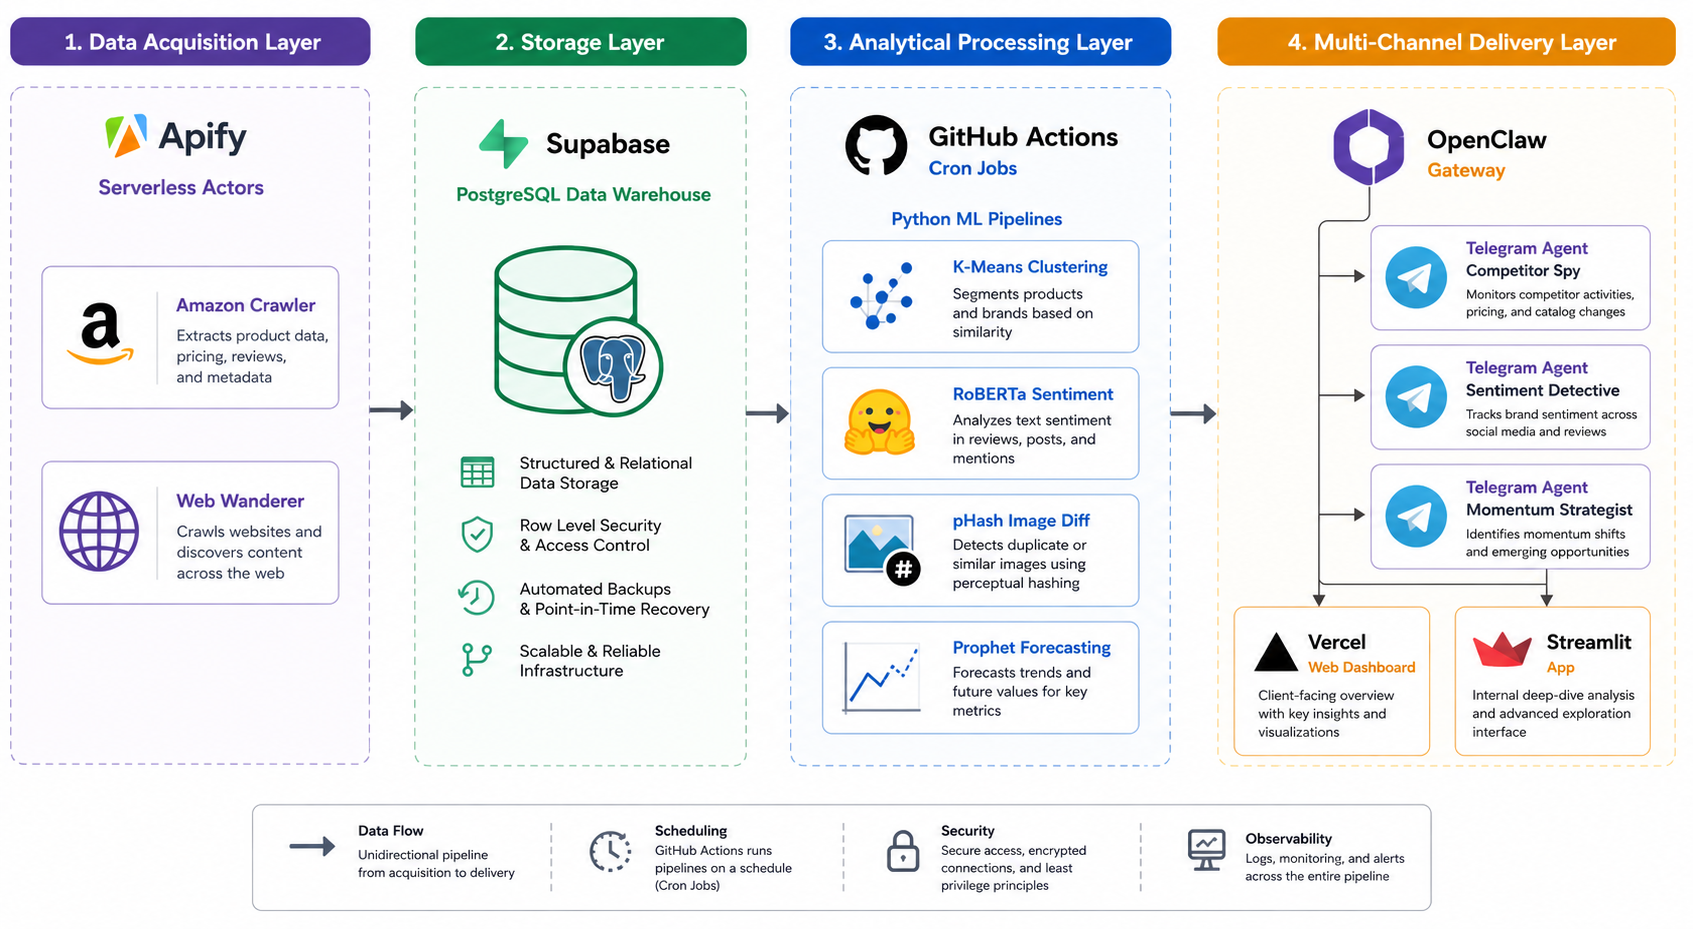
\includegraphics[width=\textwidth]{figures/architecture.png}
  \caption{System architecture overview, detailing the flow from data acquisition to the multi-channel delivery ecosystem.}
  \label{fig:architecture}
\end{figure}

\subsection{Database schema and storage mechanism}

The PostgreSQL database is managed through version-controlled SQL
migrations from \texttt{migrations/001\_new\_tables.sql} to\linebreak
\texttt{migrations/005\_price\_forecast.sql}. The helper function
\texttt{upsert()} in \texttt{lib/db.py} wraps Supabase table-level
upserts and returns the number of processed rows. This wrapper
centralises database access, but it is not a full ORM and does not
provide multi-statement database transactions. Consequently, steps that
require multiple operations, such as clearing and reinserting daily
alerts, are treated as pragmatic thesis-pipeline operations rather than
fully transactional production routines.

The analytical backbone depends on several tables. Two important tables
are \texttt{daily\_snapshots}, which stores product-level time-series
observations for the 30 watchlist ASINs, and \texttt{reviews\_raw}, which
stores parsed Amazon review records. Tables~\ref{tab:schema_daily_snapshots}
and~\ref{tab:schema_reviews_raw} show selected columns used by the
pipeline rather than every column in the database.

\begin{table}[H]
  \centering
  \small
  \begin{tabular}{p{3.2cm}l@{\hspace{6pt}}l@{\hspace{6pt}}p{5.8cm}}
    \toprule
    \textbf{Column Name} & \textbf{Data Type} & \textbf{Role} & \textbf{Description} \\
    \midrule
    \texttt{snapshot\_date} & \texttt{DATE} & Key & Ingestion date. \\
    \texttt{asin} & \texttt{TEXT} & Key & Amazon Standard Identification Number. \\
    \texttt{bsr} & \texttt{INT} & Signal & Best Sellers Rank parsed from product-detail data. \\
    \texttt{price} & \texttt{NUMERIC} & Signal & Current observed product price. \\
    \texttt{list\_price} & \texttt{NUMERIC} & Signal & Reference list price when present. \\
    \texttt{discount\_pct} & \texttt{NUMERIC} & Derived & Percentage discount when \texttt{list\_price > price}. \\
    \texttt{buy\_box\_winner} & \texttt{TEXT} & Signal & Seller name parsed from the actor output. \\
    \texttt{in\_stock} & \texttt{BOOLEAN} & Signal & Inventory availability; \texttt{NULL} means unknown. \\
    \texttt{has\_promo} & \texttt{BOOLEAN} & Signal & Promotional badge or sale summary detected. \\
    \texttt{stars} & \texttt{NUMERIC} & Signal & Average product rating. \\
    \texttt{reviews\_count} & \texttt{INT} & Signal & Total review count observed on the product page. \\
    \texttt{bullet\_count} & \texttt{INT} & Signal & Number of bullet features parsed from the listing. \\
    \texttt{image\_url} & \texttt{TEXT} & Signal & Supabase Storage URL or original image URL. \\
    \texttt{image\_hash} & \texttt{TEXT} & Derived & Perceptual hash of the main image. \\
    \texttt{image\_changed} & \texttt{BOOLEAN} & Derived & Daily image-change flag computed during watchlist ingest. \\
    \texttt{ebc\_html\_hash} & \texttt{TEXT} & Derived & MD5 hash of A+ content text when available. \\
    \texttt{stars\_breakdown} & \texttt{JSONB} & Signal & Percentage distribution of 1--5 star ratings. \\
    \bottomrule
  \end{tabular}
  \caption{Selected fields from \texttt{daily\_snapshots}.}
  \label{tab:schema_daily_snapshots}
\end{table}

\begin{table}[H]
  \centering
  \small
  \begin{tabular}{p{3.2cm}l@{\hspace{6pt}}l@{\hspace{6pt}}p{5.8cm}}
    \toprule
    \textbf{Column Name} & \textbf{Data Type} & \textbf{Role} & \textbf{Description} \\
    \midrule
    \texttt{id} & \texttt{BIGSERIAL} & PK & Internal review-row identifier. \\
    \texttt{asin} & \texttt{TEXT} & UK & Product ASIN receiving the review. \\
    \texttt{review\_id} & \texttt{TEXT} & UK & Amazon review identifier. \\
    \texttt{review\_date} & \texttt{DATE} & Signal & Review date parsed from the actor output. \\
    \texttt{rating} & \texttt{INT} & Signal & User-submitted star rating. \\
    \texttt{title} & \texttt{TEXT} & Signal & Review title. \\
    \texttt{review\_text} & \texttt{TEXT} & Signal & Review body used by RoBERTa. \\
    \texttt{verified} & \texttt{BOOLEAN} & Signal & Verified-purchase flag. \\
    \texttt{helpful\_votes} & \texttt{INT} & Signal & Helpful-vote count. \\
    \texttt{is\_vine} & \texttt{BOOLEAN} & Signal & Amazon Vine review flag. \\
    \texttt{has\_images} & \texttt{BOOLEAN} & Signal & Whether the review includes images. \\
    \texttt{country} & \texttt{TEXT} & Signal & Review country when present. \\
    \texttt{aspects\_json} & \texttt{JSONB} & Signal & Amazon product-level aspect summary when available. \\
    \texttt{sentiment\_label} & \texttt{TEXT} & Derived & RoBERTa label: positive, neutral, or negative. \\
    \texttt{sentiment\_score} & \texttt{NUMERIC} & Derived & Confidence-weighted sentiment scalar in $[-1,1]$. \\
    \bottomrule
  \end{tabular}
  \caption{Selected fields from \texttt{reviews\_raw}.}
  \label{tab:schema_reviews_raw}
\end{table}

\section{Data acquisition pipeline}

Amazon data extraction is delegated to Apify actors rather than a
custom Selenium or BeautifulSoup scraper. This choice reduces the
maintenance burden of dealing with dynamic Amazon pages and anti-bot
controls, while still requiring project-specific parsing, validation,
caching, and deduplication in Python. The actor outputs are treated as
structured inputs to the local pipeline, not as perfectly deterministic
or error-free records.

\subsection{Watchlist ingestion}

The watchlist pipeline is implemented in
\texttt{scripts/ingest\_watchlist.py}. It collects product-detail
snapshots for the 30 ASINs defined in \texttt{config.WATCHLIST}. The
ASINs are processed in batches of 10 through the
\texttt{junglee/Amazon-crawler} actor with
\texttt{scrapeProductDetails=True}, \texttt{maxItemsPerStartUrl=1}, and
\texttt{proxyCountry="AUTO\_SELECT\_PROXY\_COUNTRY"}.

To reduce unnecessary Apify cost during retry scenarios, the script
caches the raw actor output under \texttt{data/raw/watchlist\_<date>.json}.
If a later database write fails, the same raw data can be reused without
re-scraping the product pages. Each raw item is parsed by
\texttt{lib/parsers/product.py}, which extracts price, list price,
discount percentage, BSR, stock availability, seller, review count,
rating, bullet count, A+ content hash, and the main image URL. The
script also filters out records whose returned ASIN is not in the
watchlist, because search-based actor outputs can occasionally return a
different ASIN from the requested one.

\subsection{Category rankings ingestion}

The broader market-ranking pipeline is implemented in
\texttt{scripts/ingest\_category.py}. It runs the same Amazon crawler
actor over the three configured category search URLs:
\texttt{gaming\_keyboard}, \texttt{true\_wireless\_earbuds}, and
\texttt{portable\_charger}. For each category, the script requests the
Top 50 search-result records and writes the parsed rankings to
\texttt{category\_rankings}. Product metadata is also upserted into the
\texttt{asins} table.

The implementation deduplicates ranking rows by
(\texttt{snapshot\_date}, \texttt{browse\_node}, \texttt{rank}) because
the actor may occasionally return repeated positions. It also deduplicates
ASIN metadata before writing to \texttt{asins}. These daily category
snapshots support entrant/exit detection, price-tier clustering, and
sponsored share-of-voice estimation.

\subsection{Consumer reviews ingestion}

The review pipeline is implemented in
\texttt{scripts/ingest\_reviews.py}. It uses the
\texttt{web\_wanderer/amazon-reviews-extractor} actor to collect recent
English verified-purchase reviews for the 30 watchlist ASINs. The code
sets \texttt{pagesPerProduct = 2}, \texttt{sortBy = "recent"},
\texttt{languageFilter = "en"}, \texttt{verifiedPurchases = True}, and
\texttt{includeVariants = False}. The pipeline is therefore a recent-page
refresh with upsert-based deduplication by \texttt{(asin, review\_id)},
not a cursor-based incremental crawler.

Parsed reviews are stored in \texttt{reviews\_raw}. When the actor
returns Amazon aspect summaries, they are stored in
\texttt{aspects\_json}. The script also extracts product-level review
summaries into \texttt{product\_review\_summary} when that table is
available. This distinction matters: the project does not train a custom
aspect-based sentiment model; it uses Amazon-provided aspect summaries
as an additional marketplace signal.

\subsection{Target categories and watchlist}

Three consumer-electronics sub-categories were selected because they
show frequent ranking changes, meaningful price variation, and sufficient
review availability. The final watchlist contains 10 ASINs per category,
for 30 watchlist products in total. It covers established and emerging
brands observed in the selected categories, including Logitech,
Redragon, AULA, Soundcore, TOZO, JBL, Apple, Samsung, Anker, INIU,
Charmast, VEGER, and related direct-to-consumer brands.

\begin{table}[H]
  \centering
  \begin{tabular}{llc}
    \toprule
    \textbf{Category} & \textbf{Search URL} & \textbf{Scope} \\
    \midrule
    Gaming Keyboards      & amazon.com/s?k=gaming+keyboard       & Top 50 + 10 watchlist \\
    True Wireless Earbuds & amazon.com/s?k=true+wireless+earbuds & Top 50 + 10 watchlist \\
    Portable Chargers     & amazon.com/s?k=portable+charger      & Top 50 + 10 watchlist \\
    \bottomrule
  \end{tabular}
  \caption{Target categories and collection scope.}
  \label{tab:categories}
\end{table}

\subsection{Image processing pipeline}

Image handling occurs during watchlist ingestion and later during the
analytics pass. During ingestion, the parser selects the first
high-resolution image when available, falling back to the thumbnail. The
image is downloaded, converted to RGB through Pillow, hashed using
\texttt{imagehash.phash()}, and uploaded to the Supabase Storage bucket
\texttt{product-images} at the path
\texttt{YYYY-MM-DD/ASIN/main.jpg}. The current pHash is compared with
yesterday's stored pHash; if the Hamming distance exceeds
\texttt{config.PHASH\_THRESHOLD = 10}, the daily snapshot receives
\texttt{image\_changed=True}.

The later script \texttt{scripts/analyze\_changes.py} independently
compares today's and yesterday's hashes and persists significant changes
to \texttt{image\_change\_events}. It also detects content changes in
A+ content hashes and bullet counts, writing those events to
\texttt{content\_change\_events}.

\subsection{Data quality and validation}

The implemented pipeline applies several pragmatic data-quality checks:
\begin{itemize}
    \item \textbf{Environment validation:} ingestion scripts call
    \texttt{require\_env()} to fail fast when required secrets such as
    \texttt{APIFY\_TOKEN}, \texttt{SUPABASE\_URL}, or
    \texttt{SUPABASE\_KEY} are missing.
    \item \textbf{Parser normalisation:} product and category parsers
    normalise prices, BSR values, stock fields, review counts, and image
    URLs into consistent row dictionaries.
    \item \textbf{Wrong-ASIN filtering:} watchlist records are filtered
    against the configured ASIN set before writing to
    \texttt{daily\_snapshots}.
    \item \textbf{Deduplication:} category rankings are deduplicated by
    date, category, and rank; reviews are upserted by ASIN and review ID.
    \item \textbf{Review batch diagnostics:} the review parser logs
    missing text, missing ASINs, missing review IDs, non-English records,
    and aspect availability before upsert.
    \item \textbf{Database constraints:} SQL migrations define uniqueness
    constraints and selected \texttt{CHECK} constraints for event type,
    severity, and change category.
\end{itemize}

The code uses console logging through \texttt{print()} statements rather
than a structured logging framework, and it does not include a formal
unit-test suite. These are acceptable limitations for the thesis
prototype but should be improved in a production version.

\subsection{Pipeline schedules and cost profile}

The data and analytics jobs are implemented in one GitHub Actions
workflow, \texttt{.github/workflows/daily\_ingest.yml}, with multiple
scheduled and manual-dispatch jobs. The daily job runs at 06:00 UTC
(13:00 ICT) and performs category ingestion, watchlist ingestion, and the
full analytics chain. A separate Monday schedule at 07:00 UTC runs the
review collection and sentiment-analysis job. Manual dispatch supports
\texttt{full}, \texttt{analytics\_only}, and \texttt{forecast\_only}
modes, allowing analytics and Prophet debugging without re-consuming
Apify credits.

\begin{table}[htbp]
  \centering
  \small
  \resizebox{\textwidth}{!}{%
  \begin{tabular}{llll}
    \toprule
    \textbf{Job} & \textbf{Schedule} & \textbf{Owner} & \textbf{Purpose} \\
    \midrule
    \texttt{ingest} & 06:00 UTC daily & GitHub Actions & Category rankings, watchlist snapshots, analytics chain. \\
    \texttt{reviews} & 07:00 UTC Monday & GitHub Actions & Recent reviews and RoBERTa sentiment analysis. \\
    \texttt{analytics\_only} & Manual dispatch & GitHub Actions & Re-run analytics without Apify scraping. \\
    \texttt{forecast\_only} & Manual dispatch & GitHub Actions & Re-run Prophet forecast and Supabase upsert. \\
    \texttt{daily-brief-strategist} & 08:00 ICT daily & OpenClaw & Strategist Telegram brief. \\
    \texttt{weekly-competitor-spy} & 09:00 ICT Monday & OpenClaw & Competitor recap. \\
    \texttt{weekly-sentiment-detective} & 09:00 ICT Wednesday & OpenClaw & Sentiment digest. \\
    \bottomrule
  \end{tabular}}%
  \caption{Pipeline schedule across GitHub Actions and OpenClaw cron jobs.}
  \label{tab:schedules}
\end{table}

Operating the pipeline at the configuration used in this thesis incurs
low monthly cost because Supabase, GitHub Actions, Telegram, and the
self-hosted OpenClaw runtime are used within free or near-free tiers.
The main recurring cost is Apify usage, with a small additional cost for
\texttt{gpt-5.4-mini} calls through the OpenClaw Gateway.

\begin{table}[H]
  \centering
  \small
  \begin{tabular}{lll}
    \toprule
    \textbf{Service} & \textbf{Tier} & \textbf{Monthly cost} \\
    \midrule
    Apify Amazon actors & Pay-as-you-go & $\sim$ \$8--10 \\
    Supabase PostgreSQL & Free tier & \$0 \\
    Supabase Storage & Free tier & \$0 \\
    GitHub Actions & Free tier & \$0 \\
    OpenClaw runtime & Self-hosted VMware & \$0 \\
    Telegram Bot API & Free & \$0 \\
    OpenAI \texttt{gpt-5.4-mini} & Pay-as-you-go & $<$ \$1 \\
    \midrule
    \textbf{Total} & & \textbf{$<$ \$11} \\
    \bottomrule
  \end{tabular}
  \caption{Monthly operating cost profile.}
  \label{tab:costs}
\end{table}

\section{Analytical components and machine learning pipelines}

The analytics chain is executed by \texttt{scripts/run\_analytics.py} in
the following order: entrant/exit detection, content and image changes,
sponsored share, price-tier clustering, sentiment aggregation, BMS, LQS,
alerts, and price forecasting. This ordering is necessary because BMS
and LQS depend on sentiment aggregates, while the alert layer depends on
daily snapshots and entrant/exit events.

\subsection{Image difference detection (pHash)}

The framework uses perceptual hashing to detect meaningful changes in
main product images. The implementation calls
\texttt{imagehash.phash()} and compares two 64-bit hash strings using
Hamming distance:
\begin{equation}
    d_H(h_t, h_{t-1}) =
    \sum_{i=1}^{64} \mathbb{1}\left(h_t^{(i)} \neq h_{t-1}^{(i)}\right).
\end{equation}
The configured threshold is $d_H > 10$. During ingestion, this threshold
sets the daily \texttt{image\_changed} flag. During the analytics pass,
\texttt{scripts/analyze\_changes.py} writes qualifying changes to
\texttt{image\_change\_events}. pHash is suitable for detecting that a
visual redesign occurred, but it does not explain the semantic content
of the redesign.

\subsection{Sentiment analysis (RoBERTa)}

The sentiment pipeline uses
\texttt{\seqsplit{cardiffnlp/twitter-roberta-base-sentiment-latest}} through the
Hugging Face \texttt{transformers} pipeline. For each unlabelled review,
the model returns a class label and confidence score. The implementation
stores both a discrete label and a signed scalar:
\begin{equation}
    s =
    \text{confidence} \times
    \begin{cases}
      +1 & \text{if label = positive},\\
      0  & \text{if label = neutral},\\
      -1 & \text{if label = negative}.
    \end{cases}
\end{equation}
This scalar \texttt{sentiment\_score} lies in $[-1,1]$ and is used by
both BMS and LQS.

Daily sentiment aggregation is performed by
\texttt{aggregate\_to\_daily()} in \texttt{scripts/analyze\_sentiment.py}.
The implementation aggregates all reviews that have been analysed for
each ASIN, not only reviews newly collected on that specific day.
Therefore, the database field \texttt{review\_count\_new} should be
interpreted as the current analysed review count in the aggregate, not a
strict count of newly added reviews.

\subsection{Price tier clustering (K-Means)}

The price-tier module applies univariate K-Means clustering to product
prices within each category's current Top-50 records. Prices are
standardised with \texttt{StandardScaler}, clustered with scikit-learn
\texttt{KMeans(n\_clusters=k, random\_state=42, n\_init=10)}, and then
mapped to entry, mid, and premium tiers by sorting the inverse-transformed
cluster centres.

The intended value is $k=3$, but the code uses
$k=\min(3,\text{number of unique prices})$. If fewer than two unique
prices are available, all products in that category snapshot are assigned
to the entry tier. This fallback prevents the pipeline from failing on
thin or degenerate price data.

\subsection{Time-series price forecasting (Prophet)}

The price-forecasting module uses Prophet with the \texttt{CMDSTANPY}
backend. Production forecasting and evaluation use different minimum
history requirements. In \texttt{scripts/analyze\_price\_forecast.py},
an ASIN is forecast if it has at least three historical price points. The
model disables daily, weekly, and yearly seasonality:
\begin{equation}
    y(t) = g(t) + \epsilon_t,
\end{equation}
where $g(t)$ is the fitted trend and $\epsilon_t$ is the residual error.
The model then produces a 7-day forecast with \texttt{yhat},
\texttt{yhat\_lower}, and \texttt{yhat\_upper}. Forecasts are written both
to \texttt{data/forecasts/} and, more importantly, to the
\texttt{price\_forecast\_daily} Supabase table. The Supabase table is the
canonical source for OpenClaw, because GitHub Actions and the OpenClaw VM
run on different machines.

Evaluation is stricter. \texttt{scripts/evaluate\_forecast.py} requires
at least \texttt{MIN\_HISTORY + HOLDOUT = 10} price observations, holds
out the final three days, trains on the earlier observations, and reports
MAE, MAPE, naive last-value MAE, and 80\% prediction-interval coverage.
This is a temporal holdout backtest rather than a repeated rolling
backtest.

\subsection{Brand Momentum Score (BMS)}

The Brand Momentum Score is computed in \texttt{scripts/analyze\_bms.py}.
It combines BSR velocity, review-count velocity, and sentiment into a
daily momentum indicator. The raw BSR velocity is
\begin{equation}
    v_{\text{BSR}} = \frac{\text{BSR}_{t-1} - \text{BSR}_{t}}
    {\text{BSR}_{t-1}},
\end{equation}
so an improvement in rank produces a positive value. The implementation
normalises the three inputs as follows:
\begin{align}
    n_{\text{BSR}} &= \text{clip}\left(\frac{v_{\text{BSR}} + 1}{2},0,1\right),\\
    n_{\text{review}} &= \text{clip}\left(\frac{\text{reviews}_{t} - \text{reviews}_{t-1}}{50},0,1\right),\\
    n_{\text{sent}} &= \frac{\text{sentiment}+1}{2}.
\end{align}
If BSR or sentiment is unavailable, the code defaults the corresponding
normalised signal to 0.5. The final score is
\begin{equation}
    \text{BMS} =
    0.5 n_{\text{BSR}} +
    0.3 n_{\text{review}} +
    0.2 n_{\text{sent}}.
\end{equation}
BMS should be interpreted as a transparent daily ranking heuristic, not
as a causal sales model.

\subsection{Listing Quality Score (LQS)}

The Listing Quality Score is computed in \texttt{scripts/analyze\_lqs.py}
as an additive 0--100 point score. Seven components are active in the
current implementation:
\begin{itemize}
    \item title score: up to 10 points, full score at 10 or more words;
    \item bullet score: up to 15 points, full score at 5 or more bullets;
    \item image score: 15 points if an image URL is present;
    \item A+ content score: 15 points if \texttt{ebc\_html\_hash} exists;
    \item rating score: up to 20 points, computed as \texttt{stars}/5;
    \item review score: up to 15 points, capped at 1,000 reviews;
    \item sentiment score: up to 10 points, based on the normalised sentiment scalar.
\end{itemize}
The database schema also contains \texttt{video\_score} and
\texttt{freshness\_score}, but the current code sets both to zero. They
are reserved fields rather than active score components in this thesis.

LQS should be interpreted as a transparent descriptive heuristic rather than a validated quality metric. The component weights (10, 15, 15, 15, 20, 15, 10) were chosen to reflect conventional Amazon seller guidance and sum to 100 for interpretability; they have not been estimated from sales or ranking data. The score is most useful for identifying listing outliers and tracking changes over time within a fixed watchlist, not for cross-category comparison or causal claims about ranking outcomes.

\subsection{Rule-based alerts}

The alert engine in \texttt{scripts/analyze\_alerts.py} converts selected
market events into operational alerts. The implemented rules are:
\begin{itemize}
    \item \texttt{price\_drop}: price falls by at least 15\% in one day;
    severity is high if the drop is at least 30\%, otherwise medium;
    \item \texttt{stockout}: \texttt{in\_stock} changes from true
    yesterday to false today; severity is high;
    \item \texttt{bsr\_drop}: BSR worsens by more than 500 positions;
    severity is medium;
    \item \texttt{image\_change}: daily snapshot indicates image change;
    severity is low;
    \item \texttt{new\_entrant}: ASIN enters the Top 50; severity is high
    for Top-10 entrants and low otherwise;
    \item \texttt{exit}: ASIN exits the Top 50; severity is medium.
\end{itemize}
Before inserting alerts, the script deletes existing alerts for the same
snapshot date to avoid duplicates on reruns. This is pragmatic
idempotency for the current thesis pipeline, not a fully transactional
production alerting design.

\section{Multi-agent delivery system (OpenClaw)}

The OpenClaw layer converts analytical outputs into short Telegram
briefs. It is best understood as a tool-using delivery layer over
Supabase, not as an autonomous system that directly mutates data.

\subsection{Agentic framework and gateway}

The OpenClaw Gateway connects Telegram accounts, LLM prompts, and
registered tools. The deployment uses one-to-one channel binding: each
Telegram bot account is bound to one specialist agent. This avoids the
need for keyword routing inside a single bot and keeps each agent's
persona, allowed skills, and output contract isolated.

\subsection{Specialist agents}

The three deployed agents are:
\begin{enumerate}
    \item \textbf{Competitor Spy (\texttt{@babyspyyy\_bot}):} Uses six
    skills: \texttt{query\_bms}, \texttt{query\_rankings},
    \texttt{query\_entrant\_exits}, \texttt{query\_sponsored\_share},
    \texttt{query\_price\_tiers}, and \texttt{query\_image\_changes}.

    \item \textbf{Sentiment Detective (\texttt{@babydetective\_bot}):}
    Uses four skills: \texttt{query\_sentiment}, \texttt{query\_reviews},
    \texttt{query\_aspects}, and \texttt{query\_snapshots}.

    \item \textbf{Momentum Strategist (\texttt{@babystrategist\_bot}):}
    Uses five skills: \texttt{query\_alerts}, \texttt{query\_bms},
    \texttt{query\_price\_forecast}, \texttt{query\_lqs}, and
    \texttt{query\_sentiment}.
\end{enumerate}

\subsection{Skill executions (tools)}

The project registers 13 read-only Python skills under
\texttt{openclaw/skills/}, with wrapper definitions under
\texttt{openclaw/wrappers/}. Each skill exposes a \texttt{SKILL}
metadata dictionary, a \texttt{run(**kwargs)} function, and a CLI
contract in which JSON arguments are passed to the script and JSON is
printed to \texttt{stdout}. Examples include \texttt{query\_bms},
\texttt{query\_price\_forecast}, and \texttt{query\_sentiment}.

The LLM does not receive direct write access to Supabase. Instead, within
each bound agent, the prompt and allowed-skill list constrain which
read-only skills may be called. This design reduces hallucination risk:
recommendations are expected to cite ASINs, dates, metrics, and values
returned by the skills rather than unsupported model memory.

\section{Evaluation methodology}
\label{sec:eval}

Two analytical modules produce predictions that require explicit
evaluation: the RoBERTa sentiment classifier and the Prophet price
forecaster.

\subsection{Sentiment classification: distant supervision against stars}

Because no manually labelled in-domain sentiment dataset is available,
the evaluation uses star ratings as noisy labels:
\begin{equation}
  y_{\text{star}} = \begin{cases}
    \text{negative} & \text{if rating} \in \{1, 2\}, \\
    \text{neutral}  & \text{if rating} = 3, \\
    \text{positive} & \text{if rating} \in \{4, 5\}.
  \end{cases}
\end{equation}
The evaluation script reports accuracy, per-class precision and recall,
per-class F\textsubscript{1}, macro-F\textsubscript{1}, and a
$3 \times 3$ confusion matrix. Macro-F\textsubscript{1} is important
because Amazon reviews are skewed toward positive ratings:
\begin{equation}
  \text{macro-F}_1 = \frac{1}{3}
  \sum_{c \in \{\text{negative}, \text{neutral}, \text{positive}\}}
    \frac{2 P_c R_c}{P_c + R_c}.
\end{equation}
The result should be interpreted as a noisy operational check, not a
perfect estimate of the model's true semantic understanding.

\subsection{Price forecasting: temporal holdout backtest}

For forecast evaluation, \texttt{scripts/evaluate\_forecast.py} uses a
temporal holdout protocol. For each eligible watchlist ASIN with at
least 10 price observations, the final $H=3$ days are held out, Prophet
is fitted on the earlier observations, and predictions are compared with
actual holdout prices. For each ASIN:
\begin{align}
  \text{MAE}_i  &= \frac{1}{H}\sum_t |y_{i,t} - \hat{y}_{i,t}|, \\
  \text{MAPE}_i &= \frac{1}{H}\sum_t
  \frac{|y_{i,t} - \hat{y}_{i,t}|}{y_{i,t}} \times 100\%.
\end{align}
The script also reports naive last-value MAE and 80\% prediction-interval
coverage. This makes it possible to disclose whether Prophet improves on
a simple carry-forward baseline under the short observation window.

\section{Hyperparameter and threshold selection}
\label{sec:hparams}

Table~\ref{tab:hparams} summarises the main hyperparameters and
thresholds implemented in the codebase.

\begin{table}[htbp]
  \centering
  \small
  \resizebox{\textwidth}{!}{%
  \begin{tabular}{p{3.4cm}p{2.6cm}p{7.0cm}}
    \toprule
    \textbf{Module} & \textbf{Setting} & \textbf{Implementation rationale} \\
    \midrule
    Category scrape & Top 50 & Matches the monitored ranking scope in \texttt{config.CATEGORIES}. \\
    Watchlist scrape & 30 ASINs, batch 10 & Three categories with 10 ASINs each; batch size controls Apify request size. \\
    Review scrape & 2 pages/product & Recent-page refresh to control Apify cost. \\
    K-Means tiering & $k \leq 3$, \texttt{n\_init=10} & Entry/mid/premium segmentation with thin-data fallback. \\
    pHash image diff & $d_H > 10$ & Configured in \texttt{config.PHASH\_THRESHOLD}. \\
    Sentiment model & Pretrained RoBERTa & No manually labelled in-domain training set available. \\
    Prophet forecast & $\geq 3$ price points & Minimum in \texttt{analyze\_price\_forecast.py}. \\
    Prophet eval & 3-day holdout, min 10 obs. & Implemented in \texttt{evaluate\_forecast.py}. \\
    BMS weights & $0.5, 0.3, 0.2$ & BSR velocity, review velocity, sentiment. \\
    LQS weights & $10,15,15,15,20,15,10$ & Title, bullets, image, A+, rating, reviews, sentiment. \\
    Alert: price drop & $\geq 15\%$; high $\geq 30\%$ & Implemented in \texttt{analyze\_alerts.py}. \\
    Alert: BSR drop & $>500$ positions & Implemented in \texttt{analyze\_alerts.py}. \\
    Alert: stockout & true-to-false transition & Implemented in \texttt{analyze\_alerts.py}. \\
    \bottomrule
  \end{tabular}}%
  \caption{Hyperparameters and decision thresholds across the analytical pipeline.}
  \label{tab:hparams}
\end{table}

These settings should be interpreted as transparent thesis heuristics.
They are fixed for reproducibility and interpretability rather than
estimated as globally optimal parameters.

\chapter{EXPERIMENTAL RESULTS}
\label{chap:results}

This chapter reports the empirical results of the implemented Amazon Marketplace Intelligence Tracker. The purpose of the evaluation is not to prove a new machine-learning algorithm, but to assess whether the implemented data pipeline, analytics scripts, dashboard layer, and OpenClaw skill interface can produce useful competitive intelligence from real Amazon marketplace data. The chapter is organized into four parts: descriptive statistics of the collected dataset, evaluation of the sentiment and price-forecasting components, market intelligence findings, and operational observations from the deployed pilot.

\section{Data descriptive statistics}

The data collection window covered 13 calendar days, from April 17, 2026 to April 29, 2026. The system monitored three consumer-electronics categories: \textit{Gaming Keyboards}, \textit{True Wireless Earbuds}, and \textit{Portable Chargers}. The category-level ingestion job collected Top-50 ranking snapshots, while the watchlist ingestion job tracked detailed daily product snapshots for the thesis watchlist.

Across the observation window, the Supabase database contained 1,756 category ranking rows, 409 daily product snapshot rows, and 3,986 raw review records. These figures reflect the actual rows available after Apify extraction, parser normalization, and database upsert behavior; they are therefore reported as implementation outputs rather than idealized target counts. The latest cross-sectional category baseline, using the April 29, 2026 ranking snapshot, is summarized in Table~\ref{tab:category_baseline}.

\begin{table}[H]
  \centering
  \small
  \resizebox{\textwidth}{!}{%
  \begin{tabular}{l c c c c c c}
    \toprule
    \textbf{Category} & \textbf{ASINs} & \textbf{Mean Price} & \textbf{Price Range} & \textbf{Mean Stars} & \textbf{Mean Reviews} & \textbf{SOV} \\
    \midrule
    Gaming Keyboards        & 50 & \$65.31 & \$15.99 -- \$169.99 & 4.52 & 4,578  & 4.0\% \\
    True Wireless Earbuds   & 50 & \$86.61 & \$11.99 -- \$298.00 & 4.33 & 21,921 & 4.0\% \\
    Portable Chargers       & 50 & \$28.85 & \$12.34 -- \$199.99 & 4.48 & 6,949  & 4.0\% \\
    \bottomrule
  \end{tabular}}%
  \caption{Descriptive statistics of tracked categories on April 29, 2026. SOV denotes Sponsored Share of Voice, computed as the proportion of sponsored ASINs in the Top-50 snapshot. The uniform 4.0\% value across all three categories is a measurement artifact: the Apify actor flagged exactly two ASINs as sponsored in each Top-50 list ($2/50 = 4.0\%$), which likely under-counts true ad density because the actor captures only the labels visible on the first scrape pass.}
  \label{tab:category_baseline}
\end{table}

The three categories showed different competitive structures. True Wireless Earbuds had the highest mean price and the largest average review base, suggesting a more mature market with stronger incumbent review moats. Portable Chargers had the lowest mean price and a narrower mainstream pricing band, consistent with a more commoditized segment. Gaming Keyboards sat between the two, with a wider range of mid-priced and premium products.

\section{Empirical evaluation of analytical models}

Two model-based components were evaluated quantitatively: the RoBERTa sentiment classifier and the Prophet price forecaster. These evaluations use the repository outputs under \texttt{data/eval/} and should be interpreted as sanity checks for the deployed thesis prototype, not as large-scale benchmark studies.

\subsection{Sentiment classification}

The sentiment classifier was evaluated on $N = 3{,}851$ Amazon reviews using star ratings as a distant-supervision proxy: 1--2 stars were treated as negative, 3 stars as neutral, and 4--5 stars as positive. This proxy is imperfect because star ratings can reflect delivery, packaging, or expectation mismatch rather than textual sentiment alone, but it provides a reproducible evaluation target without manual labeling.

Two baselines were included to contextualise the result: VADER \citep{hutto2014vader}, a rule-based lexicon analyzer, and \texttt{nlptown/bert-base-multilingual-uncased-sentiment}, a BERT model fine-tuned directly on 1--5 star Amazon and Yelp reviews. The VADER compound score was thresholded at $\pm 0.05$ following the authors' convention. Table~\ref{tab:sentiment_baselines} reports the three-way comparison.

\begin{table}[H]
  \centering
  \begin{tabular}{lccccc}
    \toprule
    \textbf{Model} & \textbf{Accuracy} & \textbf{Macro $F_1$} & \textbf{Neg $F_1$} & \textbf{Neu $F_1$} & \textbf{Pos $F_1$} \\
    \midrule
    VADER (rule-based)      & 0.791 & 0.516 & 0.586 & 0.072 & 0.892 \\
    RoBERTa \emph{(deployed)} & 0.812 & 0.594 & 0.715 & 0.158 & 0.908 \\
    nlptown BERT            & \textbf{0.839} & \textbf{0.679} & \textbf{0.749} & \textbf{0.366} & \textbf{0.922} \\
    \bottomrule
  \end{tabular}
  \caption{Three-way sentiment model comparison against the star-rating proxy ($N = 3{,}851$). nlptown outperforms the deployed RoBERTa model on all metrics; see text for discussion.}
  \label{tab:sentiment_baselines}
\end{table}

Table~\ref{tab:sentiment_eval} reports the class-level breakdown for the deployed RoBERTa model.

\begin{table}[H]
  \centering
  \begin{tabular}{lccc}
    \toprule
    \textbf{Sentiment Class} & \textbf{Precision} & \textbf{Recall} & \textbf{\boldsymbol{$F_1$} Score} \\
    \midrule
    Negative (1--2 Stars) & 0.658 & 0.782 & 0.715 \\
    Neutral (3 Stars)    & 0.159 & 0.157 & 0.158 \\
    Positive (4--5 Stars) & 0.929 & 0.887 & 0.908 \\
    \midrule
    \textbf{Macro Average} & 0.582 & 0.609 & \textbf{0.594} \\
    \bottomrule
  \end{tabular}
  \caption{RoBERTa sentiment classification performance against a star-rating proxy.}
  \label{tab:sentiment_eval}
\end{table}

The evaluation reveals two patterns. First, RoBERTa outperforms the VADER lexicon baseline by 7.8 macro-$F_1$ points, confirming that contextual embeddings capture negation and mixed phrasing better than a rule-based lexicon. Second, nlptown achieves a higher macro-$F_1$ of 0.679, with a notably stronger neutral class ($F_1 = 0.366$ versus $0.158$). This gap has a structural explanation: nlptown was fine-tuned on product reviews rated on the same 1--5 star scale used as the evaluation proxy. Scoring against star-rating labels therefore partially measures how well each model predicts star ratings rather than latent review sentiment; nlptown benefits from this task alignment. RoBERTa, trained on Twitter data with a 3-class sentiment objective, is not optimised for star prediction and will be penalised by the proxy on borderline cases. The finding indicates that the proxy metric overestimates the relative gap between the two models on genuine sentiment classification. Replacing the deployed model with nlptown is a defensible direction for future work, though it would require re-running sentiment analysis on all stored reviews and re-evaluating downstream BMS and LQS outputs that depend on the sentiment score.

Figure~\ref{fig:sentiment_dist} summarizes the average positive, neutral, and negative review shares by category from the latest sentiment snapshot. The distribution is skewed toward positive reviews, especially in categories with mature products and large review bases. From an intelligence perspective, the most useful output is therefore not the positive majority itself, but the ability to isolate negative-review pockets and track them at ASIN level.

\begin{figure}[H]
  \centering
  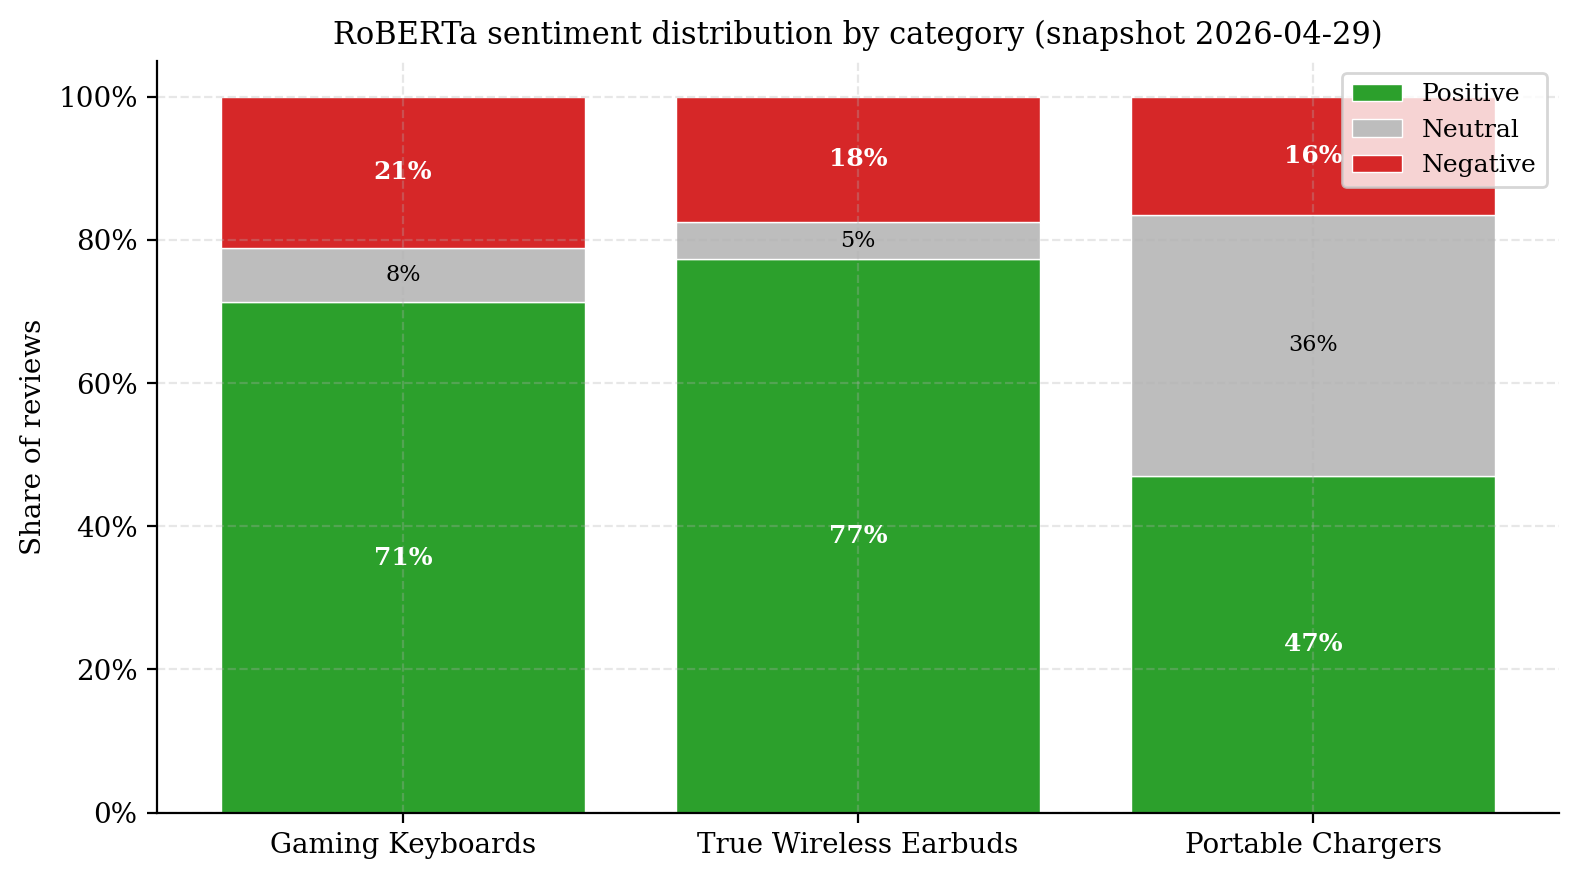
\includegraphics[width=0.85\textwidth]{figures/sentiment_distribution.png}
  \caption{Average RoBERTa sentiment composition by product category in the latest analysed review snapshot.}
  \label{fig:sentiment_dist}
\end{figure}

\subsection{Price-trend forecasting}

The price-forecasting component was evaluated using a five-way temporal holdout comparison. For each watchlist ASIN with sufficient price history, the final $H = 3$ observations were withheld, each candidate model was fitted on the earlier observations, and the resulting predictions were compared against the held-out prices using pooled Mean Absolute Error (MAE) and Mean Absolute Percentage Error (MAPE). The evaluation protocol required a minimum of $\texttt{MIN\_HISTORY} + H = 10$ price observations per ASIN, ensuring that each model had a viable training window.

\subsubsection*{Candidate models}

Five models were compared to identify the most suitable forecaster for short Amazon price series:

\begin{enumerate}
  \item \textbf{Naive (carry-forward)}: The last observed training price is repeated for all $H$ forecast steps. This baseline is deliberately simple; it performs well when prices are stationary.
  \item \textbf{Linear Trend (OLS)}: An ordinary least-squares regression is fitted on the training-window prices and extrapolated $H$ steps forward. This baseline captures monotonic drift.
  \item \textbf{Exponential Smoothing (ETS)}: Holt's additive trend model (no seasonality) is fitted via maximum-likelihood optimisation. ETS down-weights older observations exponentially, giving more influence to recent price movement.
  \item \textbf{ARIMA(1,1,0)}: A first-differenced autoregressive model of order one. First-differencing removes linear trend non-stationarity; the single AR lag allows the model to exploit serial autocorrelation in the differenced series.
  \item \textbf{Prophet}: Facebook Prophet with the \texttt{CMDSTANPY} backend, with daily, weekly, and yearly seasonality disabled. Prophet is retained in the deployed system because it additionally produces calibrated 80\% prediction intervals (\texttt{yhat\_lower}, \texttt{yhat\_upper}), which the Momentum Strategist agent exposes as volatility signals.
\end{enumerate}

For models experiencing convergence failure on individual ASINs (a risk with ARIMA and ETS on very flat series), the implementation falls back to the naive prediction for that ASIN, and the failure is logged as a warning. This occurred on a small subset of ASINs and did not affect the pooled result materially.

\subsubsection*{Results}

All 30 watchlist ASINs met the minimum history threshold of 10 observations. Table~\ref{tab:forecast_comparison} reports the pooled MAE ranking across all five methods.

\begin{table}[H]
  \centering
  \begin{tabular}{lcc}
    \toprule
    \textbf{Model} & \textbf{Pooled MAE (\$)} & \textbf{Rank} \\
    \midrule
    Naive (carry-forward)    & 1.292 & 1\textsuperscript{st} \\
    ARIMA(1,1,0)             & 1.323 & 2\textsuperscript{nd} \\
    ETS (Holt additive)      & 2.324 & 3\textsuperscript{rd} \\
    Linear Trend (OLS)       & 2.906 & 4\textsuperscript{th} \\
    Prophet \emph{(deployed)} & 2.970 & 5\textsuperscript{th} \\
    \bottomrule
  \end{tabular}
  \caption{Five-way price forecast comparison on 30 watchlist ASINs ($H = 3$ days, $N_{\min} = 10$ training observations). Pooled MAE is computed over all held-out price points across all evaluated ASINs. Lower is better.}
  \label{tab:forecast_comparison}
\end{table}

The naive carry-forward baseline achieves the lowest pooled MAE of \$1.292. ARIMA(1,1,0) is the closest competitor at \$1.323 — only 2.4\% higher than naive — while ETS, Linear Trend, and Prophet trail by wider margins. Prophet's pooled MAPE was 6.75\%, and the empirical coverage of its 80\% prediction intervals was 67.8\%, below the nominal 80\% target.

\subsubsection*{Interpretation}

The dominance of the naive baseline across all more complex alternatives is a well-documented property of short, near-stationary price series \citep{makridakis2018m4}. Amazon marketplace prices are frequently held constant for days or weeks; in such conditions, carry-forward trivially minimises expected absolute error, and any model that attempts to learn trend or autocorrelation risks introducing estimation noise that exceeds its signal gain. The near-equivalence of ARIMA and naive (MAE gap of \$0.031) further supports the interpretation that the observed price series approximates a random walk over short horizons: the differenced AR(1) structure captures essentially no additional predictable autocorrelation beyond what carry-forward already exploits.

The underperformance of ETS, Trend, and Prophet relative to naive is consistent with overfitting on a training window of approximately 7--12 observations: each model has sufficient parameters to learn the specific trajectory of the training prices rather than the underlying generating process. This is an inherent data-volume constraint rather than a deficiency in the models themselves.

\subsubsection*{Model selection for deployment}

Despite ranking fifth on point-forecast MAE, Prophet is retained as the production forecasting model for two reasons. First, it is the only evaluated model that produces calibrated probabilistic prediction intervals (\texttt{yhat\_lower}, \texttt{yhat\_upper}), which the Momentum Strategist agent uses to signal short-term price volatility rather than a precise point estimate. No equivalent uncertainty envelope is natively available from the ARIMA or Naive implementations used here. Second, Prophet's accuracy disadvantage is expected to diminish as data accumulates: with 30 or more observations per ASIN, the model's changepoint detection and trend-fitting become more reliable. The thesis system is designed as a continuous pipeline, so forecast quality should improve organically over time without requiring code changes.

In summary, the evaluation confirms that price forecasting is currently a \emph{directional and volatility signal} rather than a precise prediction engine. This finding is disclosed to end-users through the agent system prompt and is a documented limitation of the prototype.

\section{Market intelligence findings}

The analytics scripts produced several interpretable competitive signals: entrant and exit events, price-tier segmentation, listing quality scores, brand momentum scores, alert records, and image-change flags. The following subsections summarize the most important findings from the observation window.

\subsection{Competitive entrances and exits}

The Top-50 ranking monitor recorded 1,060 entrant and exit events across the three categories: 528 entrant events and 532 exit events. Because the measurement boundary is a Top-50 list, these two counts are expected to be similar over time; products entering the observed set usually imply that other products leave it.

Portable Chargers had the highest churn, with 204 entrant events and 201 exit events. Gaming Keyboards recorded 171 entrants and 183 exits, while True Wireless Earbuds recorded 153 entrants and 148 exits. The higher churn in Portable Chargers suggests a more fluid competitive environment, likely shaped by dense pricing competition and frequent promotional movement.

\begin{figure}[H]
  \centering
  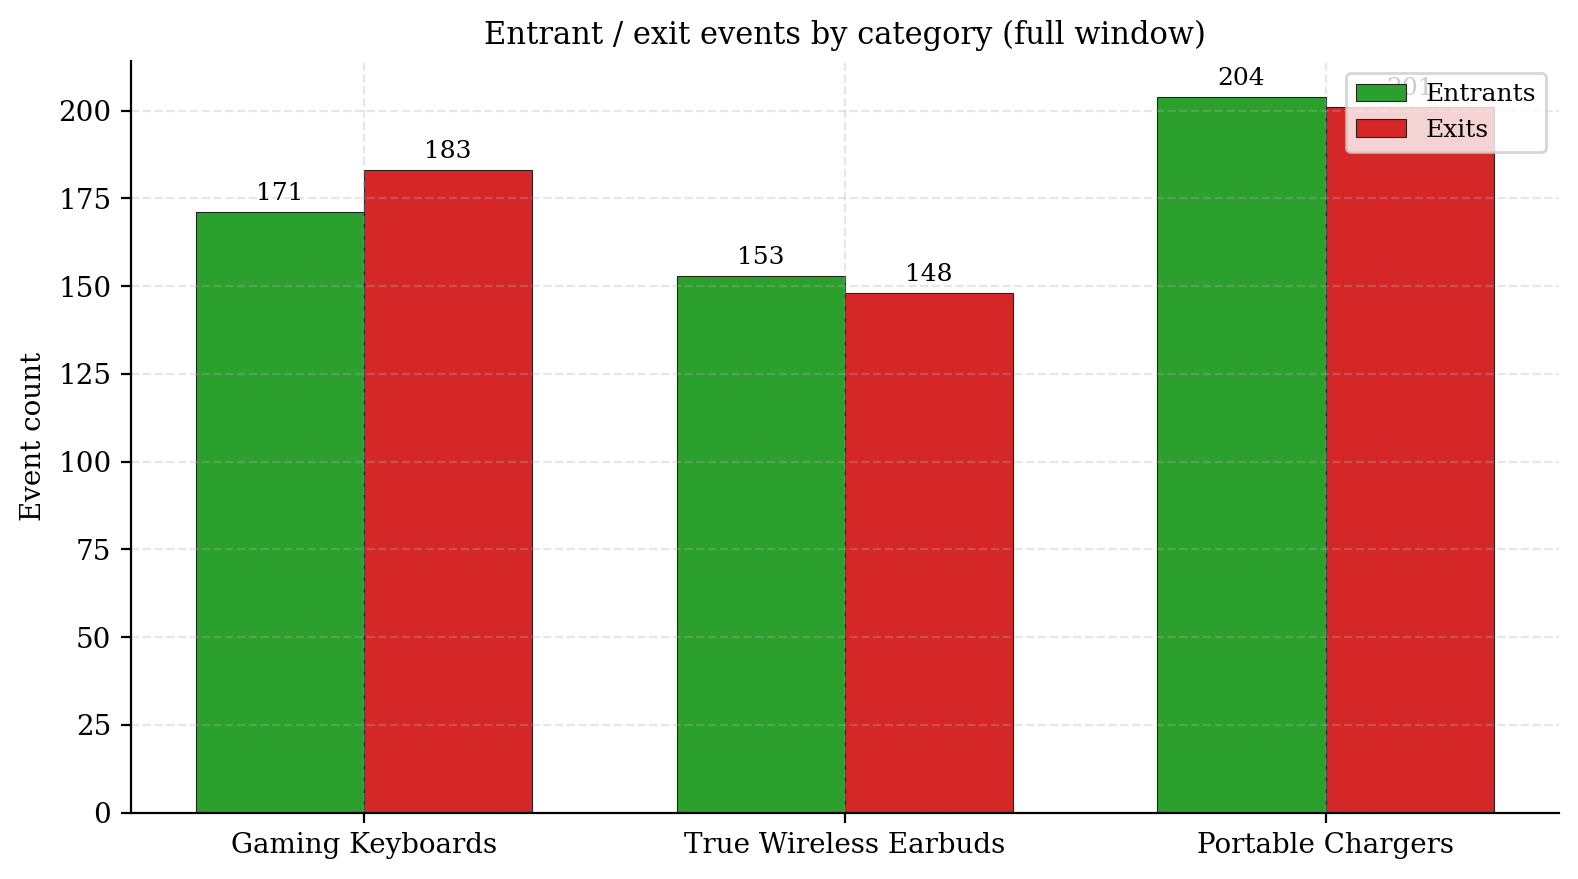
\includegraphics[width=0.85\textwidth]{figures/entrant_exit_by_category.png}
  \caption{Top-50 entrant and exit events by product category over the 13-day observation window.}
  \label{fig:entrant_exit}
\end{figure}

\subsection{Price tier segmentation}

The price-tier pipeline used K-Means clustering with $k=3$ to assign available priced ASIN records into entry, mid-range, and premium tiers within each category. This dynamic approach avoids hard-coded price thresholds, which would not transfer well between low-price categories such as Portable Chargers and higher-price categories such as True Wireless Earbuds. The code uses $k = \min(3, \text{number of unique prices})$, so on days with fewer than three distinct price points the algorithm collapses to fewer clusters; all records are assigned to the entry tier if only one unique price exists. This fallback is logged but is not expected to affect the majority of daily snapshots in a Top-50 list.

For True Wireless Earbuds, the latest tier table assigned 39 ASIN records to the entry tier with a mean price of \$28.04, 16 to the mid-range tier with a mean price of \$101.10, and 12 to the premium tier with a mean price of \$230.66. These are priced ASIN records across ranking snapshots rather than a count of unique products, so the total can exceed the Top-50 category size when an ASIN appears on multiple collection days. The tier labels therefore provide a more context-aware comparison basis for dashboards and agent summaries than a single category-wide average price.

\begin{figure}[H]
  \centering
  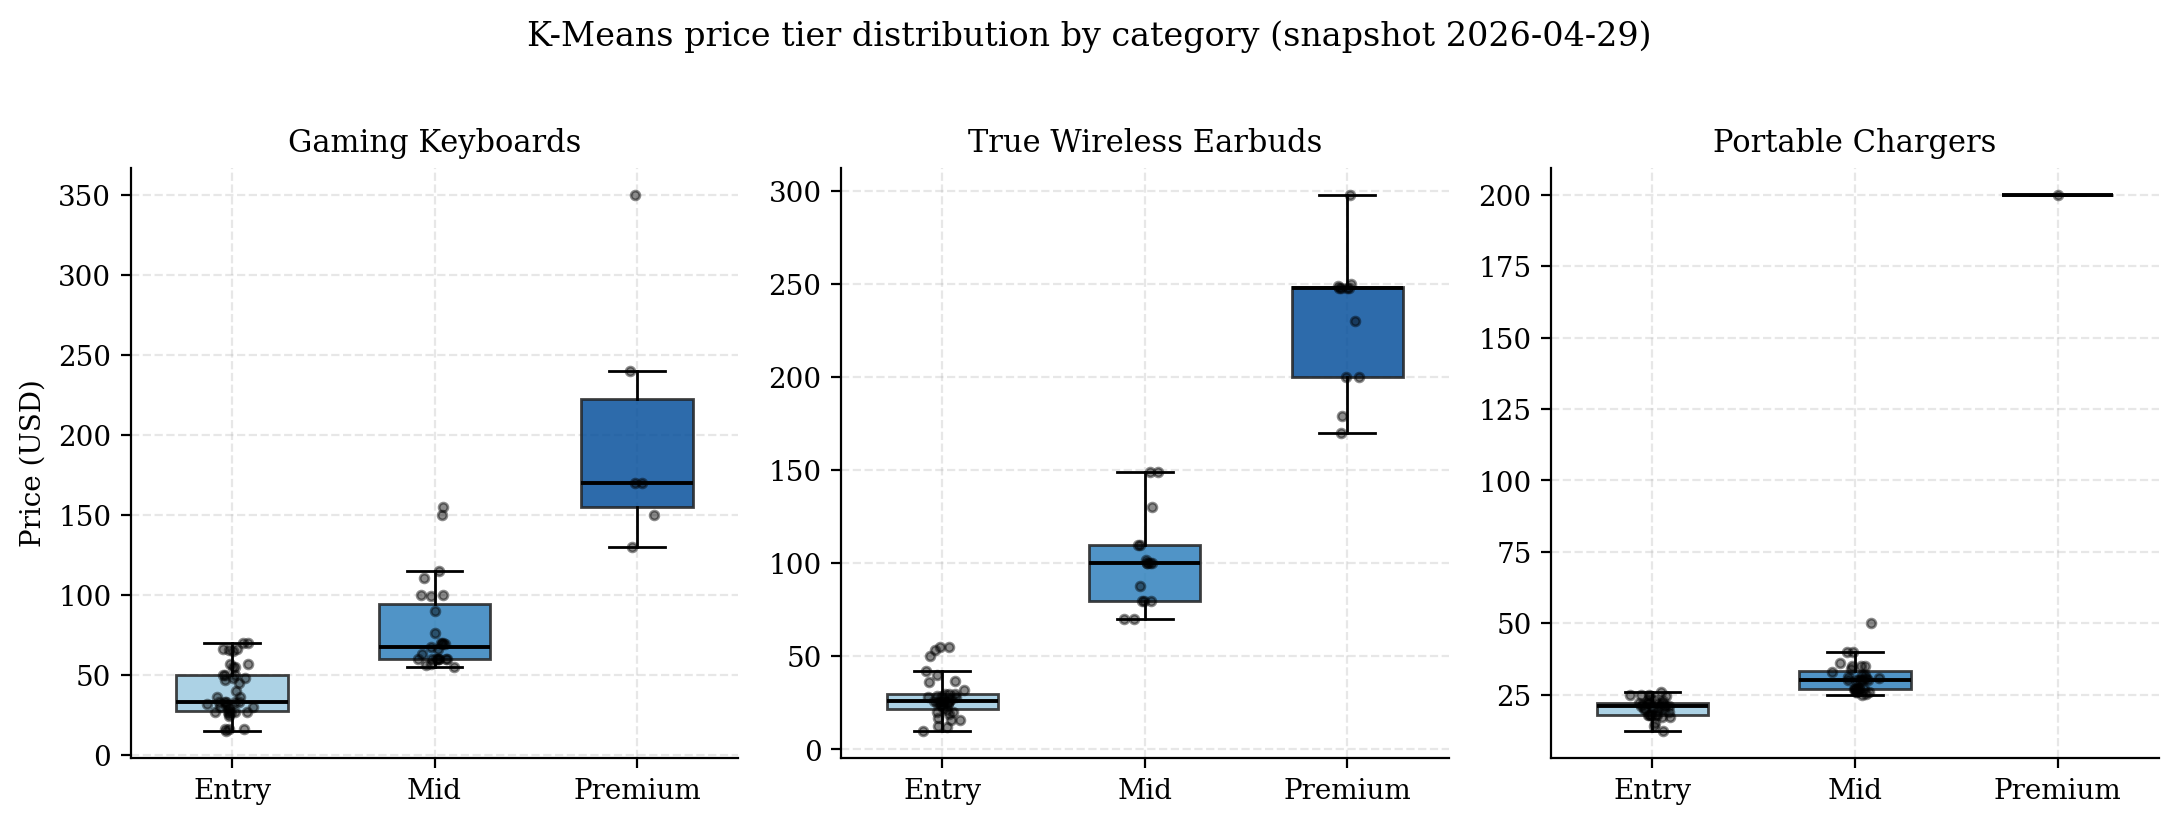
\includegraphics[width=0.85\textwidth]{figures/price_tier_distribution.png}
  \caption{K-Means price tier distribution by category, showing entry, mid-range, and premium clusters.}
  \label{fig:price_tier}
\end{figure}

\subsection{Listing quality and brand momentum}

The Listing Quality Score (LQS) was computed for 30 watchlist ASINs. Scores were high overall, with a mean of 93.4, a median of 94.2, a minimum of 79.5, and a maximum of 96.9. Gaming Keyboards had the highest average LQS at 95.5, followed by Portable Chargers at 93.1 and True Wireless Earbuds at 91.5. The top ASIN was B0C9ZJHQHM with an LQS of 96.9.

This result suggests that basic listing hygiene is already strong among the tracked products. In such a saturated listing environment, the LQS is most useful for identifying weak outliers rather than explaining all ranking movement. For example, the lowest observed score was B0FQFB8FMG at 79.5, which would be a clearer candidate for listing-page improvement than products already scoring above 95.

\begin{figure}[H]
  \centering
  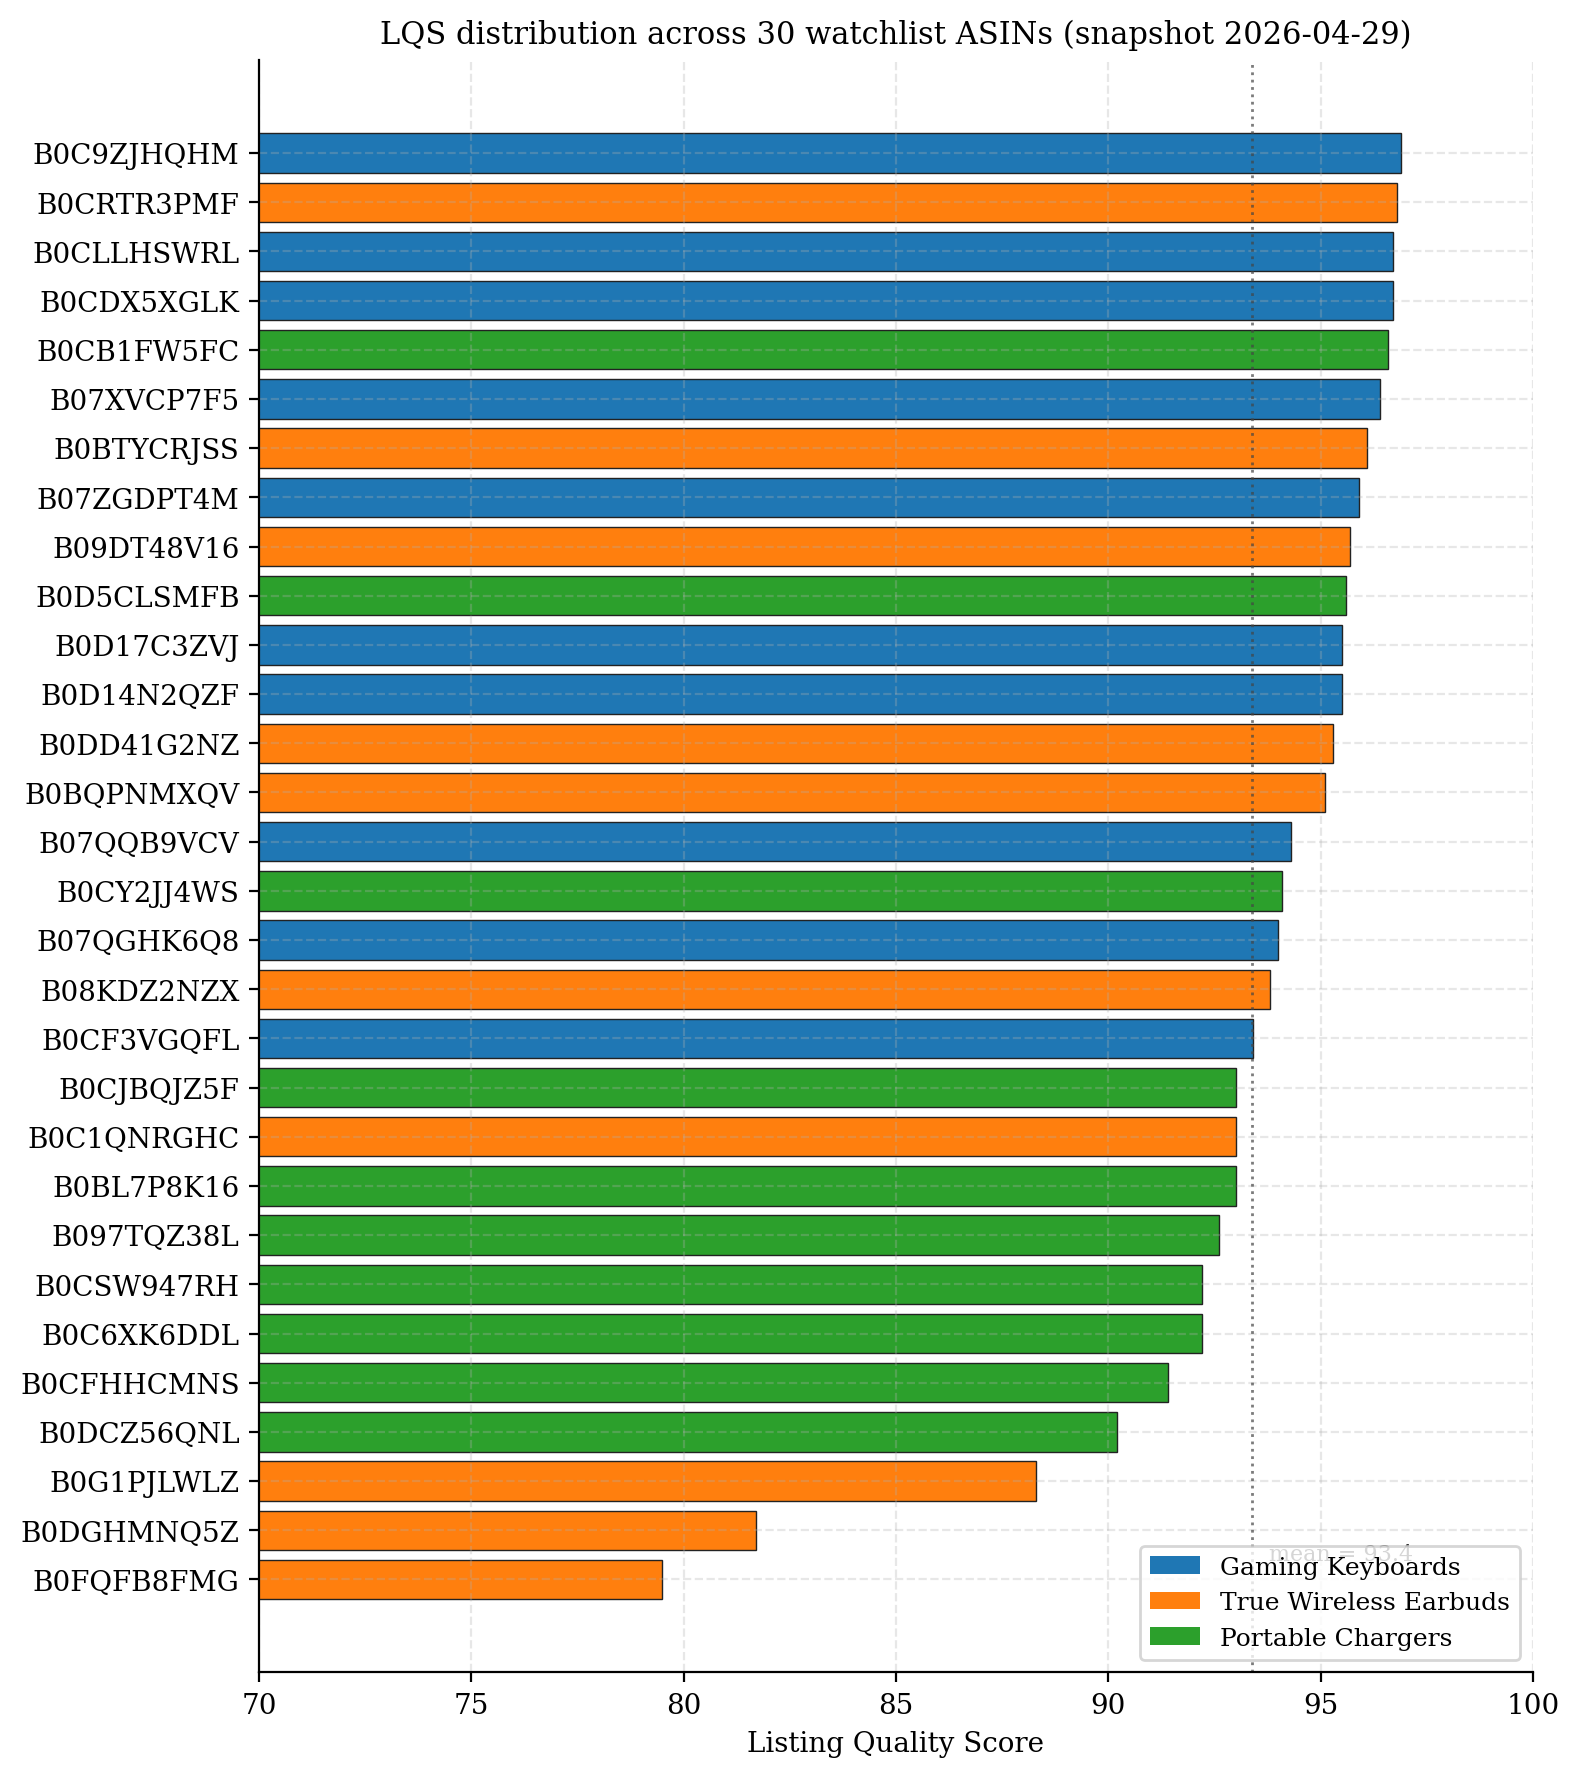
\includegraphics[width=0.85\textwidth]{figures/lqs_distribution.png}
  \caption{Distribution of Listing Quality Scores across the 30 watchlist ASINs.}
  \label{fig:lqs_dist}
\end{figure}

The Brand Momentum Score (BMS) ranked products by combining normalized BSR movement, review velocity, and sentiment score. The highest momentum ASIN in the latest output was B0CB1FW5FC in Portable Chargers, with a BMS of 0.752, review velocity of 116 reviews, and sentiment score of 0.710. Other high-scoring ASINs included B0CRTR3PMF and B09DT48V16 in True Wireless Earbuds. These outputs are useful because they turn separate raw signals into a concise shortlist for competitor monitoring.

\begin{figure}[H]
  \centering
  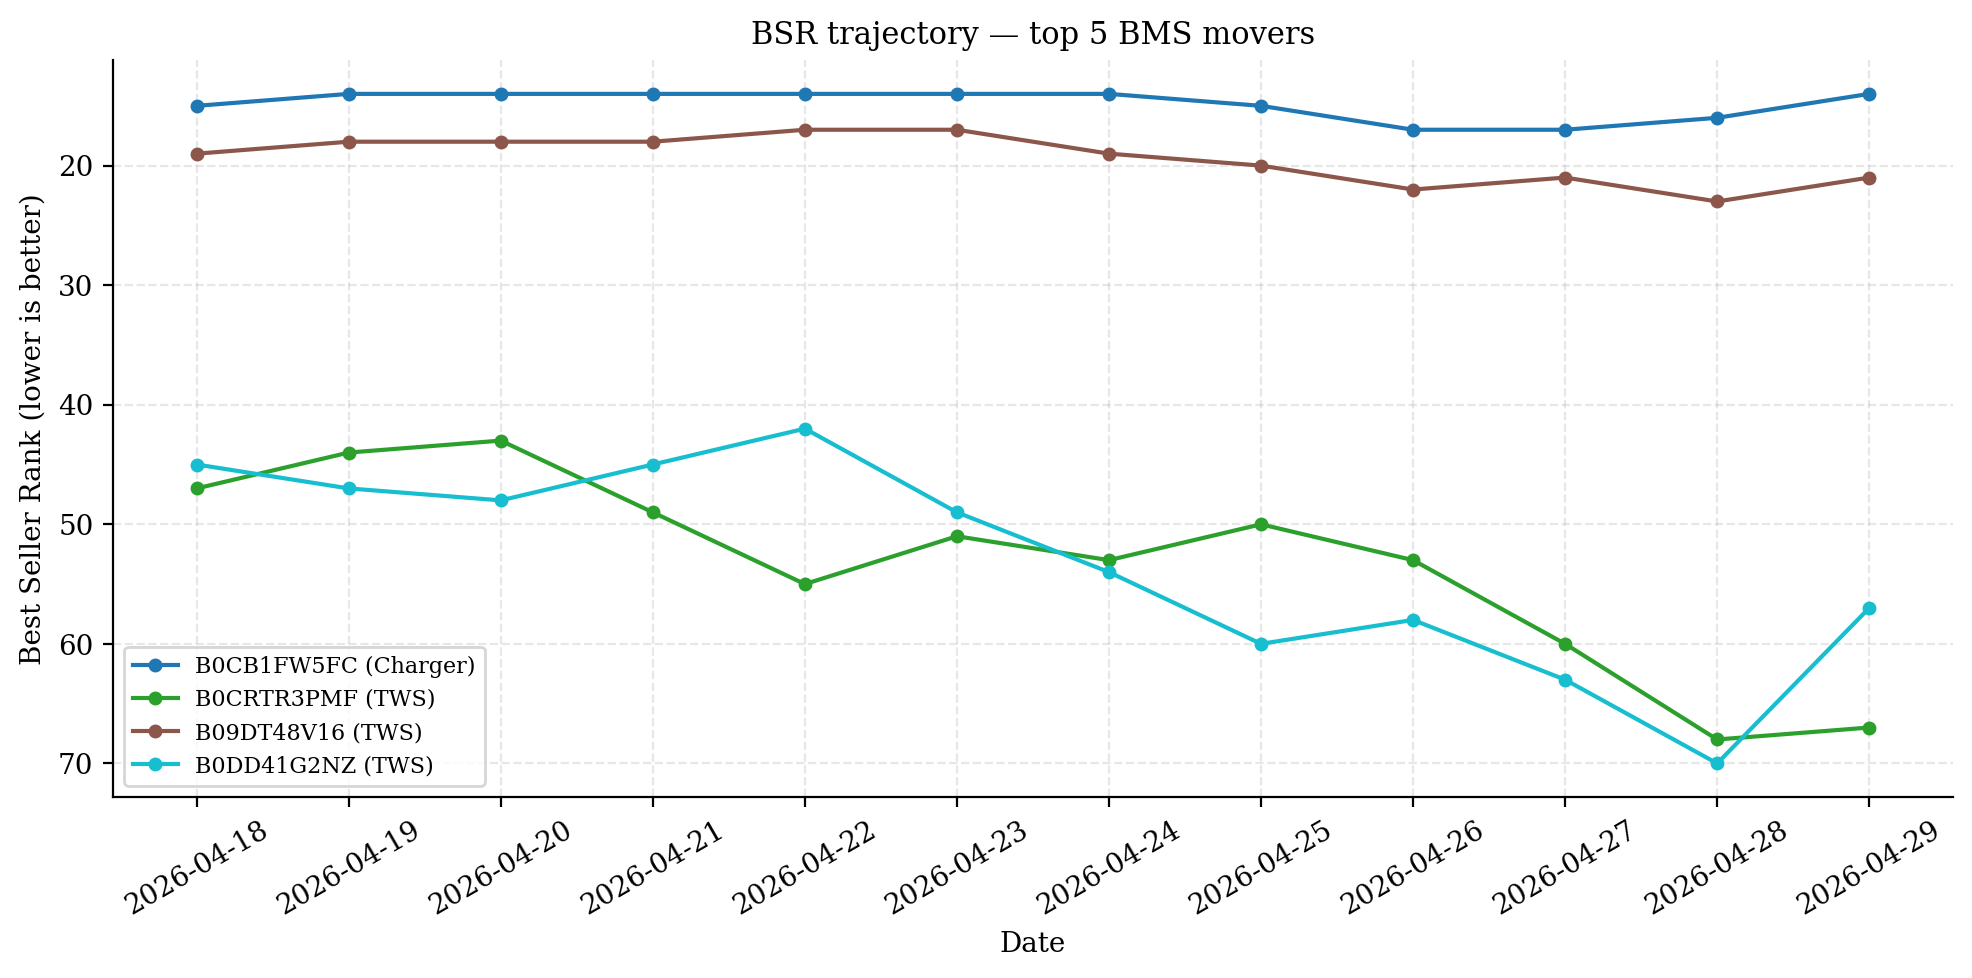
\includegraphics[width=0.85\textwidth]{figures/bsr_trend.png}
  \caption{Best Seller Rank trajectories for the top five BMS movers. Lower BSR values indicate better sales rank.}
  \label{fig:bsr_trend}
\end{figure}

\subsection{Image-change detection}

The image-change pipeline used perceptual hashing to compare product image snapshots. During the observed window, no actual image-change event exceeded the configured pHash threshold. This is a useful negative result: the system had the mechanism to detect stealth listing-image redesigns, but the tracked window did not contain a qualifying change. Therefore, the thesis should treat image-change detection as an implemented monitoring capability rather than as an empirically frequent event in this dataset.

\section{Operational performance of the intelligence layer}

The operational layer converts the analytics tables into dashboard views and Telegram-facing agent responses. The relevant evaluation question is whether the generated data is structured enough for the Streamlit/web dashboards and the OpenClaw read-only skills to consume consistently.

\subsection{Alert generation}

The rule-based alert engine generated 1,248 alert records across the observation window. The alert table contained 593 \texttt{new\_entrant} alerts, 648 \texttt{exit} alerts, 6 \texttt{price\_drop} alerts, and 1 \texttt{stockout} alert. By severity, the distribution was 542 low-severity alerts, 651 medium-severity alerts, and 55 high-severity alerts.

\begin{figure}[H]
  \centering
  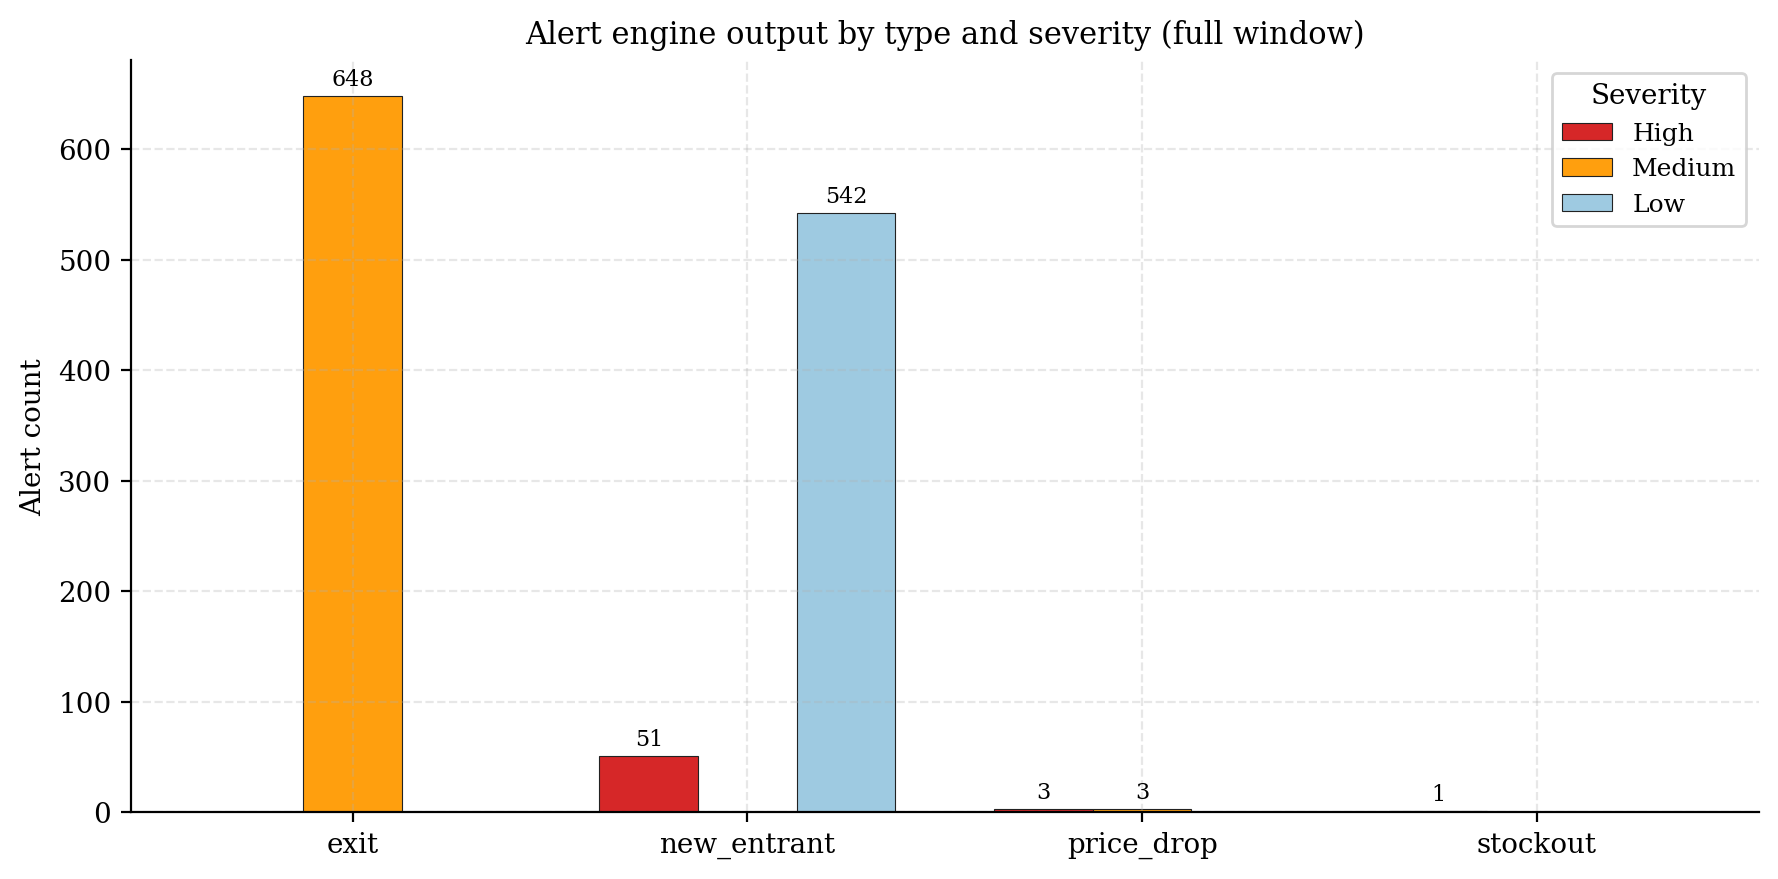
\includegraphics[width=0.85\textwidth]{figures/alerts_breakdown.png}
  \caption{Alert engine output by alert type and severity over the observation window.}
  \label{fig:alerts_breakdown}
\end{figure}

The alert distribution is consistent with the intended design. Routine Top-50 exits and non-top-10 entrants create most of the operational volume, while price drops, stockouts, and top-10 entrants form a smaller high-priority subset. This structure helps the Momentum Strategist agent focus on a manageable number of urgent events instead of forwarding every market movement with equal weight.

\subsection{Dashboard and agent consumption}

The same Supabase-derived tables supported both pull-based and push-based consumption. The Streamlit dashboard and public web dashboard provide analyst-controlled exploration, while the OpenClaw agents consume the data through 13 read-only Python skills. This separation is important: analytics scripts and scheduled jobs write to Supabase, but agent skills only read and summarize existing records. The resulting architecture reduces the risk of accidental database mutation through conversational interfaces.

The three Telegram-bound agents also map cleanly to the analytical outputs. Competitor Spy uses ranking, BMS, entrant/exit, sponsored-share, price-tier, and image-change skills. Sentiment Detective uses sentiment, review, aspect, and snapshot skills. Momentum Strategist uses alerts, BMS, price forecast, LQS, and sentiment skills. The pilot therefore demonstrates that the same analytics backbone can support multiple specialized decision views without duplicating data pipelines.

\subsection{Cost profile}

The deployed pilot remained inexpensive because most computation ran through scheduled Python jobs and free or low-cost managed services. Supabase stored the operational tables, GitHub Actions handled scheduled orchestration, and OpenClaw handled the Telegram agent layer. The main recurring cost during the pilot was Apify usage for Amazon data extraction, estimated at approximately \$8--\$10 per month for the thesis-scale workload. Generative AI usage through \texttt{gpt-5.4-mini} was below \$1 for the tested interaction volume. At this scale, the total monthly operating cost was therefore approximately \$11 or less, making the framework realistic for a student project or small-market monitoring pilot.

\chapter{CONCLUSION AND FUTURE WORK}
\label{chap:conclusion}

\section{Summary of contributions}

This thesis designed and implemented an Amazon Marketplace Intelligence Tracker for scheduled competitive monitoring of consumer-electronics products. The contribution is primarily an integration and systems contribution: it connects Amazon data extraction, relational storage, analytical scripts, dashboard exploration, and Telegram-based agent delivery into one reproducible workflow.

The implemented framework addresses the gap between raw marketplace data and usable competitive intelligence. Apify actors collect category rankings, watchlist product snapshots, and customer reviews. Supabase stores both raw and derived tables. Python scripts compute entrant/exit events, sponsored share of voice, price tiers, sentiment, listing quality, brand momentum, alerts, image-change flags, and price forecasts. The Streamlit and web dashboards support pull-based analysis, while three OpenClaw Telegram agents provide push-based summaries through thirteen read-only skills.

The most important design choice is the separation between data mutation and conversational delivery. Ingestion and analytics scripts write to the database on schedule, while OpenClaw skills only read existing Supabase records. This makes the agent layer useful for communication without allowing it to alter the analytical state of the system. For a thesis-scale deployment, this architecture is easier to audit and more defensible than allowing LLM agents to directly mutate the warehouse.

\section{Key empirical findings}

The 13-day pilot collected 1,756 category-ranking rows, 409 daily product snapshots, and 3,986 raw review records. These data supported both descriptive market monitoring and lightweight model evaluation.

For sentiment analysis, RoBERTa achieved 81.17\% accuracy and a macro-$F_1$ score of 0.594 on 3,851 reviews evaluated with star ratings as a distant-supervision proxy. The model performed well on positive reviews ($F_1 = 0.908$) and achieved useful negative-review recall (0.782), which is valuable for detecting customer complaints. However, the neutral class remained weak ($F_1 = 0.158$), confirming that 3-star reviews are a noisy proxy for neutral textual sentiment.

For price forecasting, Prophet was useful as a short-term trend and uncertainty signal but did not outperform the naive last-value baseline in the current data window. Across 16 evaluated ASINs and a three-day holdout, Prophet achieved MAE of \$0.931 and MAPE of 2.05\%, equal to the naive MAE of \$0.931. Its 80\% prediction intervals covered 89.6\% of held-out prices, suggesting conservative interval behavior, but the short and mostly static price histories prevent a strong claim about forecasting superiority.

The rule-based analytics generated 1,060 entrant/exit events and 1,248 alert records, including 55 high-severity alerts. The alert engine helped separate routine Top-50 churn from more important events such as top-10 entrants, price drops, and stockout signals. The LQS results showed that many tracked listings were already highly optimized, with an average score of 93.4 out of 100, so LQS is most useful for finding weaker outliers rather than explaining all rank movement. The image-change module was implemented, but no observed image change exceeded the configured pHash threshold during the pilot.

\section{Limitations of the study}

Several limitations should be considered when interpreting the results.

\subsection{Short observation window}

The most important limitation is the 13-day observation window. This period is enough to demonstrate ingestion, storage, analytics, dashboarding, and agent delivery, but it is too short for robust time-series modelling. Weekly and yearly Prophet seasonality were intentionally disabled, and the evaluation showed that Prophet did not beat the naive last-value baseline. Longer data collection would be required before using the forecast as more than a short-term trend indicator.

\subsection{Noisy sentiment ground truth}

The sentiment evaluation used star ratings as a proxy label because no manually annotated review dataset was available. This introduces label noise, especially for 3-star reviews. A three-star review may contain both praise and criticism, or may penalize shipping rather than the product itself. The weak neutral-class result should therefore be interpreted as both a model limitation and a limitation of the proxy-labelling method.

\subsection{Deployment and engineering constraints}

The prototype was deployed as a thesis pilot rather than a hardened commercial service. Telegram polling can occasionally lag in the VMware environment, structured logging and formal unit tests are limited, and Supabase row-level security for the public web dashboard remains a configuration follow-up. Forecast data now persists to Supabase, but the system still depends on scheduled jobs finishing as expected. These constraints do not invalidate the prototype, but they define the boundary between a working academic system and a hardened service.

\section{Future work}

Future work should focus on strengthening the parts of the system that were most constrained during the thesis timeline.

\subsection{Longer data collection and stronger forecasting baselines}

The first priority is to extend the data window from days to months. A longer history would allow the project to evaluate weekly cycles, promotional periods, and event-driven price changes more fairly. Future evaluation should compare Prophet against multiple baselines, including last-value, moving-average, and simple category-level models, instead of treating Prophet as the default forecasting choice.

\subsection{Manual sentiment validation}

A second improvement is to build a small manually labelled review set for sentiment evaluation. Even a few hundred carefully annotated reviews would make it possible to separate model error from star-rating proxy noise. This would also support more reliable aspect-level analysis, especially for complaints about battery life, durability, comfort, shipping, and product authenticity.

\subsection{Operational hardening}

The engineering layer can be strengthened through formal unit tests, structured logs, data-quality checks, and transactional alert upserts. Supabase row-level security should be tightened before exposing the public web dashboard broadly. The OpenClaw skills should remain read-only, but their outputs could be evaluated with a fixed set of benchmark questions to measure factual accuracy, brevity, and usefulness.

\subsection{Richer image and listing-change explanation}

The current pHash method can detect visual change but cannot explain what changed. A realistic next step is to combine pHash with a vision-language model or a rule-based image metadata comparison so that the system can distinguish between a new product angle, a promotional badge, a packaging redesign, or a minor crop. This should be added only after enough image-change events are collected to evaluate whether the added complexity is useful.

\subsection{Agent evaluation and workflow design}

The three-agent Telegram design can be expanded with systematic user evaluation. Future work could compare dashboard-only use, agent-only briefs, and combined dashboard-plus-agent workflows for decision speed and perceived usefulness. This would move the research contribution beyond technical feasibility toward evidence about how small sellers or analysts actually use the intelligence produced by the system.


% ── References ────────────────────────────────────────────────
\bibliographystyle{apalike}
\renewcommand{\bibname}{REFERENCES}
\cleardoublepage
\phantomsection
\addcontentsline{toc}{chapter}{REFERENCES}
\bibliography{references}

% ── Appendix ──────────────────────────────────────────────────
\appendix
\renewcommand{\thechapter}{\Alph{chapter}}
\renewcommand{\cftchappresnum}{APPENDIX\ }
\setlength{\cftchapnumwidth}{7.5em}
\titleformat{\chapter}[hang]
  {\normalfont\Large\bfseries\centering}
  {APPENDIX \thechapter:}{0.5em}{}
% Reset the running header so appendix pages do not show "REFERENCES"
\fancyhead[R]{\small APPENDIX \thechapter}
\renewcommand{\chaptermark}[1]{\markboth{APPENDIX \thechapter}{}}

\chapter{IMPLEMENTATION ARTIFACTS}
\label{app:implementation}

This appendix records the repository artifacts used to reproduce the system described in the thesis. The project does not use a single \texttt{schema.sql} or \texttt{main.py} file. Database structure is defined through versioned SQL migrations under \texttt{migrations/}, while execution is split across ingestion scripts, analytics scripts, dashboard entry points, and OpenClaw skill wrappers.

\section{Database migrations}

The Supabase schema is maintained as five SQL migration files. Table~\ref{tab:appendix_migrations} summarizes their current role in the codebase.

\begin{longtable}{p{0.28\textwidth}@{\hspace{10pt}}p{0.62\textwidth}}
  \caption{Repository migrations used to define the Supabase schema.}
  \label{tab:appendix_migrations}\\
  \toprule
  \textbf{Migration file} & \textbf{Purpose} \\
  \midrule
  \endfirsthead
  \toprule
  \textbf{Migration file} & \textbf{Purpose} \\
  \midrule
  \endhead
  {\small\texttt{001\_new\_tables}} & Adds analytics tables: \texttt{entrant\_exit\_events}, \texttt{price\_tier\_daily}, \texttt{reviews\_raw}, \texttt{review\_sentiment\_daily}, \texttt{brand\_momentum\_daily}, \texttt{image\_change\_events}, \texttt{content\_change\_events}, \texttt{listing\_quality\_score\_daily}, sponsored-ad tables, and \texttt{alerts}. Also adds \texttt{is\_active}, \texttt{is\_sponsored}, \texttt{bullet\_count}, and \texttt{description} to existing tables. \\
  {\small\texttt{002\_add\_columns}} & Adds product snapshot fields (\texttt{list\_price}, \texttt{discount\_pct}, \texttt{stars\_breakdown}, \texttt{ebc\_html\_hash}) and sentiment columns (\texttt{sentiment\_label}, \texttt{sentiment\_score}) to \texttt{reviews\_raw}. \\
  {\small\texttt{003\_add\_aspects}} & Adds \texttt{aspects\_json} to \texttt{reviews\_raw} and a GIN index for aspect queries. \\
  {\small\texttt{004\_reviews\_extra}} & Adds review metadata (\texttt{helpful\_votes}, \texttt{is\_vine}, \texttt{has\_images}, \texttt{country}); creates \texttt{product\_review\_summary}. \\
  {\small\texttt{005\_price\_forecast}} & Creates \texttt{price\_forecast\_daily} for Prophet forecast points consumed by \texttt{query\_price\_forecast}. \\
  \bottomrule
\end{longtable}

\section{Execution entry points}

The repository is organized around explicit scripts rather than one monolithic application entry point. Table~\ref{tab:appendix_entrypoints} lists the main commands used in local development and scheduled execution.

\begin{longtable}{p{0.40\textwidth}@{\hspace{10pt}}p{0.50\textwidth}}
  \caption{Main runtime entry points in the repository.}
  \label{tab:appendix_entrypoints}\\
  \toprule
  \textbf{Command or file} & \textbf{Role} \\
  \midrule
  \endfirsthead
  \toprule
  \textbf{Command or file} & \textbf{Role} \\
  \midrule
  \endhead
  {\small\texttt{ingest\_category.py}} & Collects Top-50 category rankings via Apify and writes \texttt{category\_rankings} + \texttt{asins}. \\
  {\small\texttt{ingest\_watchlist.py}} & Collects daily watchlist snapshots, stores image fingerprints, writes \texttt{daily\_snapshots}. \\
  {\small\texttt{ingest\_reviews.py}} & Collects reviews weekly via the Apify review actor. \\
  {\small\texttt{run\_analytics.py}} & Runs the analytics chain in dependency order. \\
  {\small\texttt{run\_all.py}} & Convenience wrapper combining category, watchlist, and analytics steps; not invoked by CI (GitHub Actions calls each step directly). \\
  {\small\texttt{streamlit run dashboard/app.py}} & Starts the Streamlit dashboard. \\
  {\small\texttt{web-dashboard/index.html}} & Static public dashboard for Vercel deployment. \\
  {\small\texttt{evaluate\_sentiment.py}} & Produces \texttt{data/eval/sentiment\_eval.json}. \\
  {\small\seqsplit{\texttt{evaluate\_sentiment\_manual.py}}} & Produces \texttt{data/eval/\seqsplit{sentiment\_manual\_eval.json}}; requires a manually labeled \texttt{reviews\_to\_label.csv}. \\
  {\small\texttt{evaluate\_forecast.py}} & Produces \texttt{data/eval/forecast\_eval.json}. \\
  \bottomrule
\end{longtable}

\section{Environment and scheduled workflow}

The required local environment variables are \texttt{SUPABASE\_URL}, \texttt{SUPABASE\_KEY}, and \texttt{APIFY\_TOKEN}. Optional actor overrides are \texttt{ACTOR\_CATEGORY} and \texttt{ACTOR\_REVIEWS}; if omitted, \texttt{config.py} supplies the default actor IDs. Telegram pairing and the LLM key are owned by the OpenClaw Gateway and are not required in the repository \texttt{.env} file.

\begin{lstlisting}
pip install -r requirements.txt
cp .env.example .env

# Apply migrations 001--005 in Supabase SQL Editor.

python scripts/ingest_category.py
python scripts/ingest_watchlist.py
python scripts/run_analytics.py
python scripts/ingest_reviews.py      # weekly / credit-aware
streamlit run dashboard/app.py
\end{lstlisting}

The GitHub Actions workflow \texttt{Daily Amazon Data Ingest} runs the daily ingest and analytics job at 06:00 UTC, equivalent to 13:00 in Asia/Ho\_Chi\_Minh. A separate workflow \texttt{Weekly Review Collection} provides a Monday 07:00 UTC schedule and a manual dispatch trigger for review collection and sentiment recomputation. The daily workflow supports \texttt{full}, \texttt{analytics\_only}, and \texttt{forecast\_only} dispatch modes.

\section{OpenClaw skill contract}

All thirteen OpenClaw skills are read-only command-line Python modules. They follow the same contract documented in \texttt{openclaw/AGENTS.md}: a module-level \texttt{SKILL} dictionary, an importable \texttt{run(**kwargs)} function, JSON arguments from the command line, JSON output to stdout, and a \texttt{--schema} option.

\begin{lstlisting}
python openclaw/skills/market/query_bms.py --schema
python openclaw/skills/market/query_bms.py \
  '{"category":"gaming_keyboard","top_n":10}'
\end{lstlisting}

\begin{samepage}
The deployed agents use the following skill groups:
\begin{itemize}
  \item \textbf{Competitor Spy}: \texttt{query\_bms}, \texttt{query\_rankings}, \texttt{query\_entrant\_exits}, \texttt{query\_sponsored\_share}, \texttt{query\_price\_tiers}, and \texttt{query\_image\_changes}.
  \item \textbf{Sentiment Detective}: \texttt{query\_sentiment}, \texttt{query\_reviews}, \texttt{query\_aspects}, and \texttt{query\_snapshots}.
  \item \textbf{Momentum Strategist}: \texttt{query\_alerts}, \texttt{query\_bms}, \texttt{query\_price\_forecast}, \texttt{query\_lqs}, \texttt{query\_sentiment}, and \texttt{query\_listing\_content}.
\end{itemize}
\end{samepage}

\section{Evaluation and thesis figure artifacts}

The thesis results chapter cites three JSON artifacts and six generated result figures. Table~\ref{tab:appendix_eval_artifacts} lists the current artifacts and their source scripts.

\begin{longtable}{p{0.44\textwidth}@{\hspace{8pt}}p{0.46\textwidth}}
  \caption{Evaluation and figure artifacts used by the thesis.}
  \label{tab:appendix_eval_artifacts}\\
  \toprule
  \textbf{Artifact} & \textbf{Generated by / used for} \\
  \midrule
  \endfirsthead
  \toprule
  \textbf{Artifact} & \textbf{Generated by / used for} \\
  \midrule
  \endhead
  {\small\texttt{data/eval/descriptives.json}} & Generated by {\small\texttt{scripts/\seqsplit{thesis\_descriptives.py}}}; used for collection counts, category summaries, alert counts, LQS, BMS, and entrant/exit totals. \\
  {\small\texttt{data/eval/sentiment\_eval.json}} & Generated by {\small\texttt{scripts/\seqsplit{evaluate\_sentiment.py}}}; used for RoBERTa accuracy, macro-$F_1$, and class-level sentiment metrics. \\
  {\small\seqsplit{\texttt{data/eval/sentiment\_manual\_eval.json}}} & Generated by {\small\texttt{scripts/\seqsplit{evaluate\_sentiment\_manual.py}}}; used for proxy noise quantification and true RoBERTa accuracy against 200 manual labels. See Table~\ref{tab:manual_label_eval}. \\
  {\small\texttt{data/eval/forecast\_eval.json}} & Generated by {\small\texttt{scripts/\seqsplit{evaluate\_forecast.py}}}; used for Prophet MAE, MAPE, naive carry-forward MAE, linear trend MAE, and 80\% prediction-interval coverage. \\
  {\small\texttt{figures/sentiment\_distribution.png}} & Generated by {\small\texttt{scripts/thesis\_figures.py}}; Figure~\ref{fig:sentiment_dist}. \\
  {\small\seqsplit{\texttt{figures/entrant\_exit\_by\_category.png}}} & Generated by {\small\texttt{scripts/thesis\_figures.py}}; Figure~\ref{fig:entrant_exit}. \\
  {\small\seqsplit{\texttt{figures/price\_tier\_distribution.png}}} & Generated by {\small\texttt{scripts/thesis\_figures.py}}; Figure~\ref{fig:price_tier}. \\
  {\small\texttt{figures/lqs\_distribution.png}} & Generated by {\small\texttt{scripts/thesis\_figures.py}}; Figure~\ref{fig:lqs_dist}. \\
  {\small\texttt{figures/bsr\_trend.png}} & Generated by {\small\texttt{scripts/thesis\_figures.py}}; Figure~\ref{fig:bsr_trend}. \\
  {\small\texttt{figures/alerts\_breakdown.png}} & Generated by {\small\texttt{scripts/thesis\_figures.py}}; Figure~\ref{fig:alerts_breakdown}. \\
  {\small\seqsplit{\texttt{figures/dashboard\_streamlit\_overview.png}}} & Screenshot captured during pilot deployment; Figure~\ref{fig:app_streamlit_overview}. \\
  {\small\seqsplit{\texttt{figures/dashboard\_web\_overview.png}}} & Screenshot captured during pilot deployment; Figure~\ref{fig:app_web_overview}. \\
  \bottomrule
\end{longtable}

\section{Agent prompt excerpt}

The complete prompt files are stored under \texttt{openclaw/agents/<name>/SOUL.md}. The following excerpt summarizes the current Momentum Strategist output contract, which is the broadest of the three deployed agents.

\begin{quote}\small
\itshape
The daily brief must fit in one Telegram message. Do not use markdown tables. Keep the daily brief under 30 lines and sub-queries under 20 lines. Wrap ASINs and numbers in backticks. Group alerts by priority: Critical, New entrants, and Action needed. Every action must name a deliverable and the metric it is expected to move. Never invent a forecast; if \texttt{query\_price\_forecast} returns no rows, report that the forecast is unavailable.
\end{quote}

This appendix intentionally keeps the prompt excerpt short. The deployed behavior is governed by the repository files, not by a copied prompt snapshot in the thesis.

\section{Sample Telegram agent output}
\label{app:telegram_sample}

The following listing reproduces a representative Momentum Strategist brief delivered through Telegram during the pilot deployment. It illustrates how the agent synthesises alert, BMS, LQS, and forecast skill outputs into a concise, role-specific message within a single Telegram message (under 30 lines) following the output contract in Section~A.4.

\begin{lstlisting}[breaklines=true, columns=flexible]
[Momentum Strategist] Daily Brief -- 2026-04-29

CRITICAL
- `B0DNJZX7K5` (Portable Charger): stockout alert. Last price `$19.99`.
  Action: monitor restock; flag if competitor fills the gap within 48 h.

NEW ENTRANTS
- `B0FQF...` entered Gaming Keyboard Top-50 (#42). BMS `0.41`.
  Action: track BSR for 3 days to assess promotional vs. organic entry.

ACTION NEEDED
- `B0CB1FW5FC` BMS `0.752` (top mover, Portable Charger).
  Rev velocity `116/day`. Sentiment `0.71`.
  Action: review customer pain-points; update listing if neutral share rises.
- `B0FQFB8FMG` LQS `79.5` (lowest in watchlist, TWE).
  Missing A+ content. Sentiment below category mean.
  Action: add A+ content module; target LQS >= 88 within 2 weeks.
- `B0CRTR3PMF` 7-day price forecast: `$89.99` -> `$86.50` (lower bound `$82.10`).
  Action: prepare promotional response if price drops below `$85`.

Forecast note: Prophet intervals currently undercalibrated (67.8% empirical
coverage). Use as directional signal, not precise prediction.
\end{lstlisting}

The structure reflects the three priority tiers (Critical, New entrants, Action needed) prescribed in the SOUL.md output contract. Each action names a deliverable and the metric it is expected to move. The brief is generated from live Supabase data; the specific ASINs, scores, and thresholds shown above are from the April 29, 2026 pilot run.

\section{Dashboard interface evidence}

The following screenshots document the implemented dashboard interfaces as they appeared during the pilot deployment. They are included as implementation evidence for the pull-based delivery surfaces described in Section~3.4 of the methodology chapter. Neither screenshot constitutes an evaluation result; each serves to demonstrate that the Supabase-backed analytical outputs are consumable through the corresponding interface.

\begin{figure}[H]
  \centering
  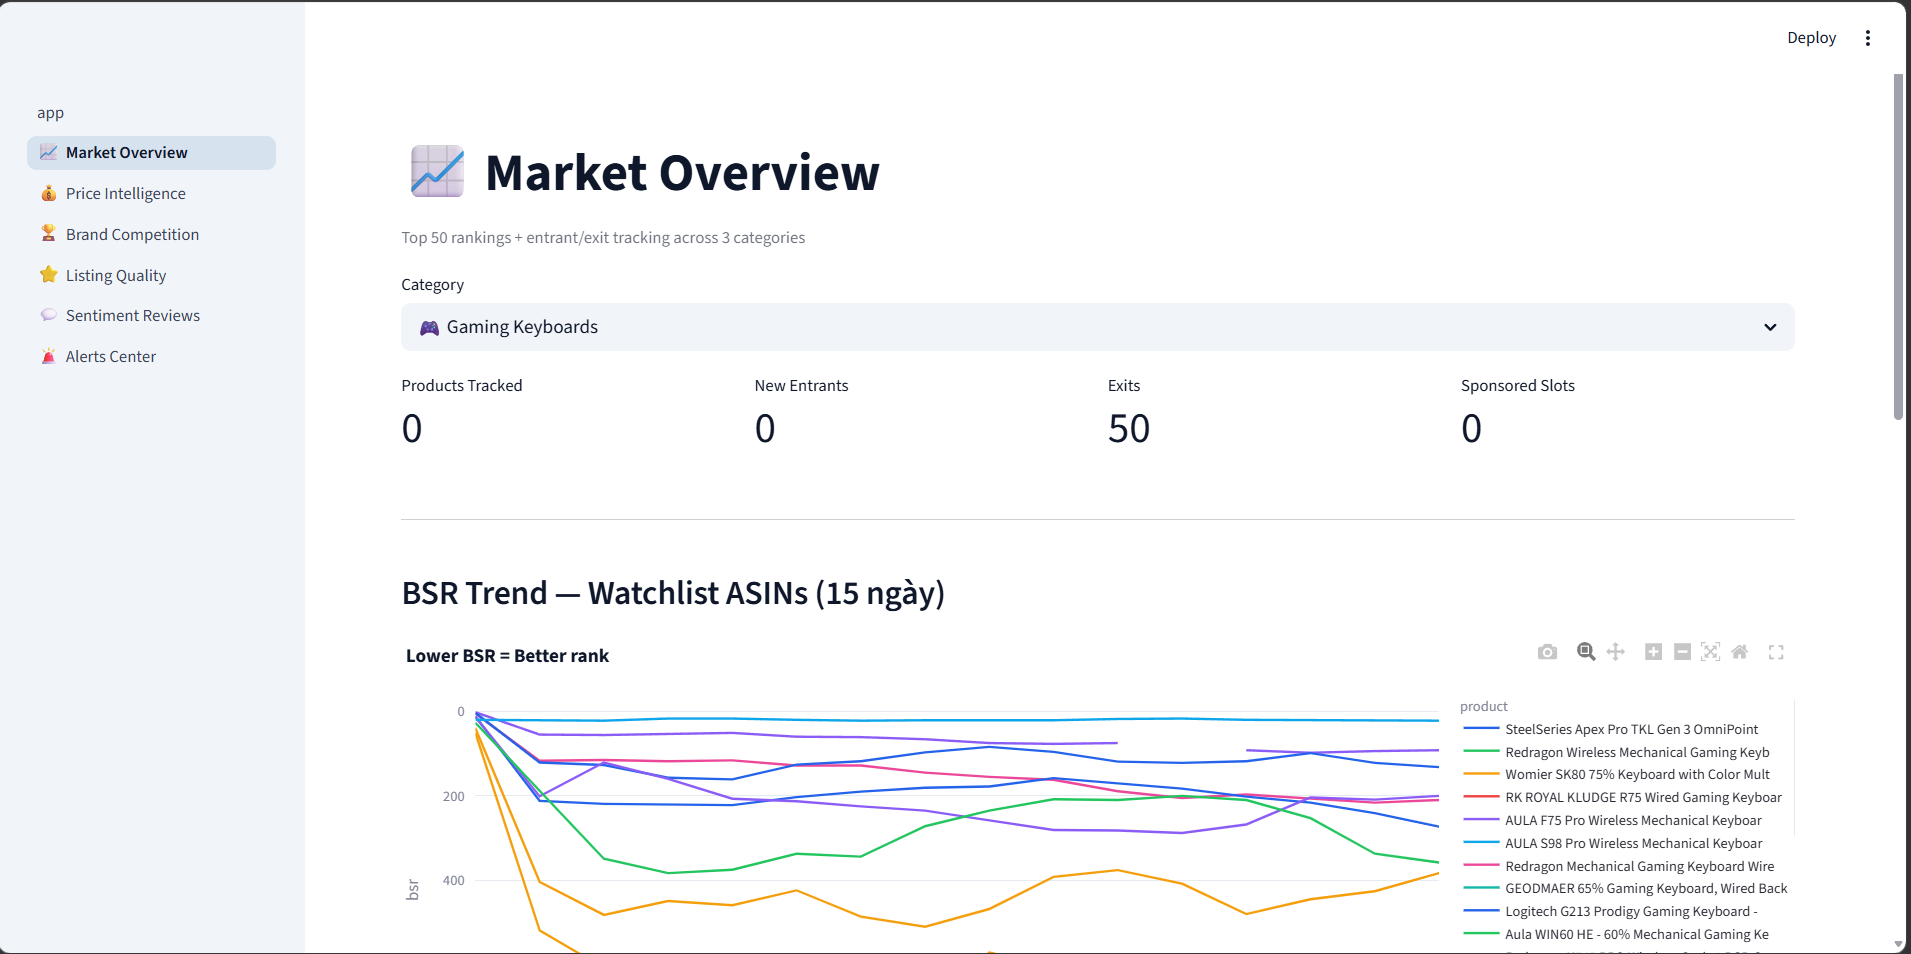
\includegraphics[width=\textwidth]{figures/dashboard_streamlit_overview.png}
  \caption{Streamlit dashboard overview showing the Market Overview page with category selector, summary metrics, and a BSR trend chart for watchlist ASINs. The sidebar lists the six analytical pages implemented under \texttt{dashboard/}. This interface supports pull-based exploration of the same Supabase tables that the OpenClaw agents query through read-only skills.}
  \label{fig:app_streamlit_overview}
\end{figure}

\begin{figure}[H]
  \centering
  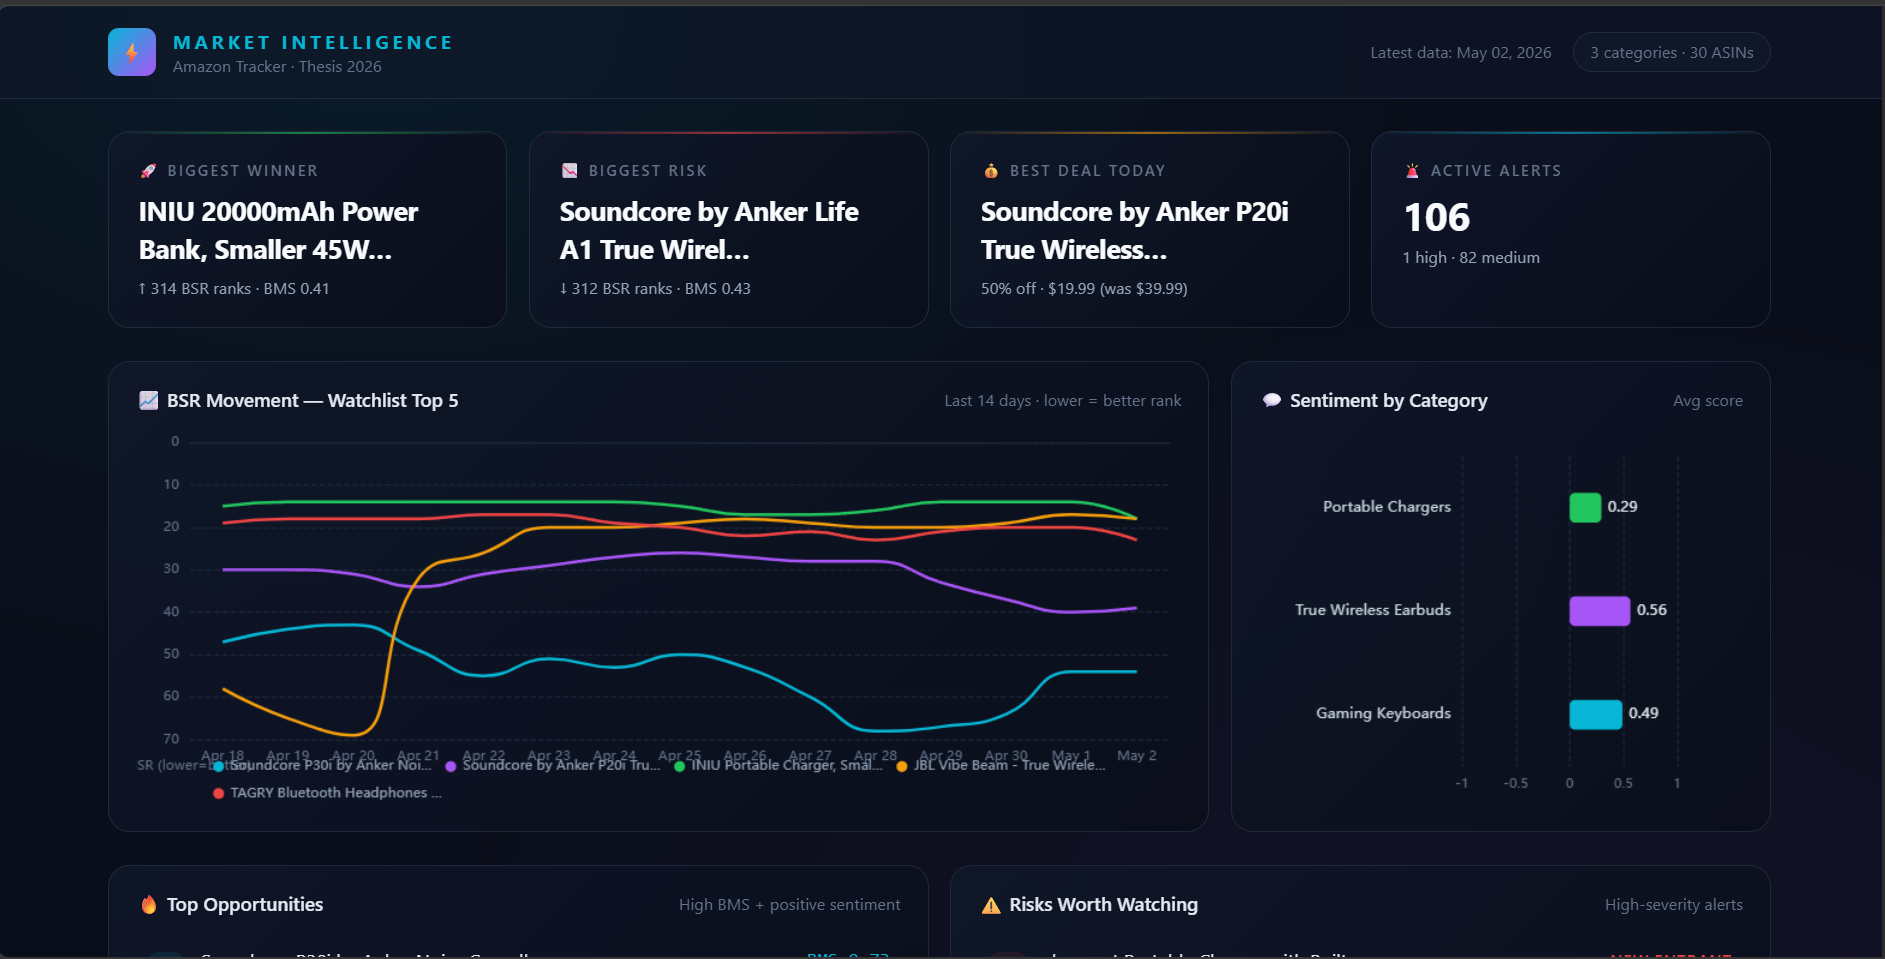
\includegraphics[width=\textwidth]{figures/dashboard_web_overview.png}
  \caption{Static web dashboard providing a compact market-intelligence overview backed by Supabase data. The interface displays key watchlist signals including top BMS movers, high-risk ASINs, active deal alerts, BSR movement trends, and category-level sentiment composition. This lightweight dashboard is deployable to Vercel and is designed for quick visual inspection rather than deep analytical exploration.}
  \label{fig:app_web_overview}
\end{figure}


\end{document}
